\documentclass{aomart}

\usepackage[T1]{fontenc}
\usepackage[nopatch=footnote]{microtype}
\usepackage{amssymb,mathtools}
\usepackage{bm}
\usepackage{aliascnt}
\usepackage{enumitem}
\usepackage{graphicx}
\usepackage{booktabs}
\usepackage{array}
\usepackage[nameinlink,noabbrev]{cleveref}

\allowdisplaybreaks
\hyphenpenalty=10000
\exhyphenpenalty=10000
\tolerance=2500
\emergencystretch=4em

\makeatletter
\def\@setsubjects{%
  \let\@subjects\@empty
  \ifx\@primarysubjects\@empty\else
    \edef\@subjects{Primary:~\@primarysubjects}%
  \fi
  \ifx\@secondarysubjects\@empty\else
    \ifx\@primarysubjects\@empty
      \edef\@subjects{Secondary:~\@secondarysubjects}%
    \else
      \edef\@subjects{\@subjects, Secondary:~\@secondarysubjects}%
    \fi
  \fi
  \ifpdf
    \hypersetup{pdfsubject=\@subjects}%
  \fi
  \if@aom@oldkeywords\else
    \@footnotetext{AMS Classification:~\@subjects.}%
  \fi
}
\makeatother

\setlist[enumerate]{topsep=4pt,itemsep=2pt}
\setlist[itemize]{topsep=4pt,itemsep=2pt}

\newtheorem{theorem}{Theorem}[section]
\newaliascnt{proposition}{theorem}
\newtheorem{proposition}[proposition]{Proposition}
\aliascntresetthe{proposition}
\newaliascnt{lemma}{theorem}
\newtheorem{lemma}[lemma]{Lemma}
\aliascntresetthe{lemma}
\newaliascnt{corollary}{theorem}
\newtheorem{corollary}[corollary]{Corollary}
\aliascntresetthe{corollary}
\theoremstyle{definition}
\newaliascnt{definition}{theorem}
\newtheorem{definition}[definition]{Definition}
\aliascntresetthe{definition}
\newaliascnt{example}{theorem}
\newtheorem{example}[example]{Example}
\aliascntresetthe{example}
\newaliascnt{standardfact}{theorem}
\newtheorem{standardfact}[standardfact]{Standard Fact}
\aliascntresetthe{standardfact}
\theoremstyle{remark}
\newaliascnt{remark}{theorem}
\newtheorem{remark}[remark]{Remark}
\aliascntresetthe{remark}

\crefname{theorem}{theorem}{theorems}
\crefname{proposition}{proposition}{propositions}
\crefname{lemma}{lemma}{lemmas}
\crefname{corollary}{corollary}{corollaries}
\crefname{definition}{definition}{definitions}
\crefname{example}{example}{examples}
\crefname{standardfact}{standard fact}{standard facts}
\crefname{remark}{remark}{remarks}

\newcommand{\CC}{\mathbb C}
\newcommand{\RR}{\mathbb R}
\newcommand{\ZZ}{\mathbb Z}
\newcommand{\NN}{\mathbb N}
\newcommand{\Hcal}{\mathcal H}
\newcommand{\Acal}{\mathcal A}
\newcommand{\Bcal}{\mathcal B}
\newcommand{\Ccal}{\mathcal C}
\newcommand{\Dcal}{\mathcal D}
\newcommand{\Ecal}{\mathcal E}
\newcommand{\Fcal}{\mathcal F}
\newcommand{\Gcal}{\mathcal G}
\newcommand{\Lcal}{\mathcal L}
\newcommand{\Mcal}{\mathcal M}
\newcommand{\Ocal}{\mathcal O}
\newcommand{\Pcal}{\mathcal P}
\newcommand{\Qcal}{\mathcal Q}
\newcommand{\Rcal}{\mathcal R}
\newcommand{\Scal}{\mathcal S}
\newcommand{\Tcal}{\mathcal T}
\newcommand{\Ucal}{\mathcal U}
\newcommand{\Vcal}{\mathcal V}
\newcommand{\End}{\operatorname{End}}
\newcommand{\Hom}{\operatorname{Hom}}
\newcommand{\Ran}{\operatorname{Ran}}
\newcommand{\Ker}{\operatorname{Ker}}
\newcommand{\Spec}{\operatorname{Spec}}
\newcommand{\Tr}{\operatorname{Tr}}
\newcommand{\tr}{\operatorname{tr}}
\newcommand{\rank}{\operatorname{rank}}
\newcommand{\diag}{\operatorname{diag}}
\newcommand{\dist}{\operatorname{dist}}
\newcommand{\id}{\mathrm{id}}
\newcommand{\e}{\mathrm e}
\newcommand{\ii}{\mathrm i}
\newcommand{\dd}{\,\mathrm d}
\newcommand{\one}{\bm 1}
\newcommand{\ket}[1]{\left|#1\right\rangle}
\newcommand{\bra}[1]{\left\langle#1\right|}
\newcommand{\norm}[1]{\left\lVert#1\right\rVert}
\newcommand{\abs}[1]{\left\lvert#1\right\rvert}
\newcommand{\ip}[2]{\left\langle#1,#2\right\rangle}
\newcommand{\ad}{\operatorname{ad}}
\newcommand{\Ad}{\operatorname{Ad}}
\newcommand{\Ob}{\operatorname{Ob}}
\newcommand{\ob}{\mathfrak o}
\newcommand{\HS}{\mathrm{HS}}
\newcommand{\phys}{\mathrm{phys}}

\graphicspath{{figures/}}

\title[Quantum packet calculus]{Quantum Packet Calculus, Symmetry, Effective Dynamics, and Continuum Towers}
\author[Komorebi P.]{Komorebi P.}
\subject{primary}{msc2020}{81P45}
\subject{secondary}{msc2020}{81P70}
\subject{secondary}{msc2020}{81Q70}
\subject{secondary}{msc2020}{47A40}
\subject{secondary}{msc2020}{81T25}
\keyword{quantum symmetry}
\keyword{quantum channel}
\keyword{error correction}
\keyword{Feshbach map}
\keyword{reflection positivity}
\keyword{spectral dimension}
\keyword{constraint algebra}
\copyrightnote{}
\doinumber{}

\pdfstringdefDisableCommands{\let\unskip\relax}
\hypersetup{
  pdftitle={Quantum Packet Calculus, Symmetry, Effective Dynamics, and Continuum Towers},
  pdfauthor={Komorebi P.},
  pdfsubject={Finite quantum packets, symmetry sectors, circuit paths, channels, error correction, effective dynamics, Euclidean transfer, and continuum criteria}
}

\begin{document}
\begin{abstract}
A finite quantum system becomes packet resolved once a complete family of orthogonal projectors is chosen. We develop the resulting calculus for states, gates, Hamiltonians, channels, code spaces, and geometric transfer. Finite group characters give isotypic packets, while cyclic charges give selection rules and tensor fusion. Circuits admit exact path expansions and block conservation laws. Moving packets are transported by the Kato connection, and a time dependent estimate identifies the off packet part of the geometric Hamiltonian. Two sided operator packets resolve density matrices and channels. Covariant channels preserve coherence order, and their Choi matrices inherit the same symmetry. The Knill Laflamme condition is expressed as vanishing of a compression obstruction, yielding orthogonal syndromes and exact recovery. Schur Feshbach elimination gives spectral equivalence, a dissipative self energy in the upper half plane, and a positive definite memory kernel. Positive transfer matrices give finite reflection positivity. Discrete tori converge at fixed diffusion time to the continuum heat trace and spectral dimension. Constraint closure is measured in the quotient by the constraint span. Exact and approximate continuum tower theorems are proved under bounded hypotheses. Unbounded field theoretic and gravitational conclusions are stated as separate requirements.
\end{abstract}
\maketitle
\thispagestyle{plain}

\section{Introduction}\label{sec:introduction}

Quantum mechanics repeatedly uses the same operation. A Hilbert space is split into sectors, an operator is resolved between those sectors, and the pieces are propagated or recombined. Symmetry sectors, eigenspaces, syndrome spaces, adiabatic subspaces, and retained model spaces are familiar examples. This article treats them as instances of one finite packet calculus.

The elementary coordinate object is a complete family of orthogonal projectors
\[
P_aP_b=\delta_{ab}P_a,
\qquad
\sum_{a\in I}P_a=I.
\]
Every vector has packet coordinates \(P_a\psi\). Every operator has transfer blocks
\[
A_{ba}=P_bAP_a.
\]
These identities are simple. Their value appears when the same coordinates are used across representation theory, circuits, channels, error correction, effective dynamics, and geometric limits.

Finite dimensional quantum information and operator theory supply the standard background \cite{NielsenChuang2010,Watrous2018,Bhatia1997}. Finite group projectors come from character theory \cite{Serre1977,FultonHarris1991}. Moving spectral subspaces and geometric phase originate in the work of Kato, Berry, Wilczek, and Zee \cite{Kato1950,Kato1995,Berry1984,WilczekZee1984}. Completely positive maps and quantum dynamical semigroups are treated in \cite{Stinespring1955,Choi1975,Kraus1983,Lindblad1976}. Exact error correction is governed by the Knill Laflamme condition \cite{KnillLaflamme1997,SchumacherNielsen1996,BenyKempfKribs2007}. Projection methods and hidden state memory are linked by the Feshbach, Nakajima, and Zwanzig constructions \cite{Feshbach1958,Nakajima1958,Zwanzig1960,BravyiDiVincenzoLoss2011}.

The first part begins with quantum seeds. A state is cyclic only relative to a declared observable algebra. For an algebra in multiplicity form, the local orbit dimension is controlled by the rank of a coefficient matrix. This recovers the relation between Schmidt rank and the dimension reached by local operations. The finite group section then constructs central isotypic projectors. Cyclic symmetry gives a sharper charge selection rule. An operator with charge \(q\) can move a state only from packet \(j\) to packet \(j+q\).

A circuit is resolved by inserting the identity between successive gates. This produces a sum over packet paths. The target probability contains diagonal path terms and interference between distinct paths. Symmetry can remove entire path families before any matrix multiplication is performed. Unitarity gives exact row and column relations among the transfer blocks.

The moving packet section treats time dependent projectors. The canonical generator
\[
K(t)=\sum_a\dot P_a(t)P_a(t)
\]
is skew adjoint and transports every packet. In the moving frame, the physical Hamiltonian acquires the geometric term \(-\ii W(t)^*\dot W(t)\). A leakage estimate shows that the relevant off packet coupling is not \(QHP\) alone. It is
\[
Q(t)\bigl(H(t)-\ii K(t)\bigr)P(t).
\]
This is the exact finite distinction between following a moving subspace and remaining in a fixed one.

Density matrices require two packet labels. The superoperators
\[
\Pcal_{ab}(X)=P_aXP_b
\]
form a complete orthogonal packet system on Hilbert Schmidt operator space. Dephasing is the diagonal projection. Every channel has input and output superblocks, with the same composition law as ordinary matrix blocks. A covariant channel preserves the isotypic packets of the conjugation action. In the cyclic case these are coherence orders. The Choi matrix carries the equivalent symmetry under \(U\otimes\overline U\).

Error correction is expressed through compression to a code. Let \(P\) be the code projector. The class of \(PAP\) modulo scalar multiples of \(P\) is the obstruction to making \(A\) invisible inside the code. The Knill Laflamme criterion says that this obstruction vanishes for every product \(E_a^*E_b\) from the error family. Diagonalizing the resulting positive coefficient matrix produces orthogonal syndrome packets and an explicit recovery on the error span.

The effective dynamics section returns to ordinary Hilbert space packets. Schur complementation gives the exact retained resolvent and a frequency dependent self energy. The same hidden block gives a causal memory kernel in time. For a self adjoint hidden Hamiltonian, the self energy has a fixed sign in the upper half plane, and the time kernel is positive definite. Uniform spectral separation gives direct bounds that can be carried through a refinement tower.

The geometric part has two finite components. A positive transfer matrix gives a reflection positive Hankel kernel and reconstructs a nonnegative Hamiltonian through its logarithm. A finite Laplacian gives a heat trace and a scale dependent spectral dimension. The article proves fixed time convergence from periodic lattices to the continuum torus. Poisson summation then gives the continuum small time dimension.

Constraint closure needs a different obstruction. If \(C_a\) are self adjoint constraints and \(P_{\phys}\) projects onto their common kernel, then
\[
P_{\phys}[C_a,C_b]P_{\phys}=0
\]
holds automatically. This compression cannot test closure. The correct finite obstruction is the class of \([C_a,C_b]\) in the quotient of \(\End(\Hcal)\) by the span of the constraints. Vanishing means that the constraint span is closed under commutators.

The last part gives two bounded continuum tower theorems. Exact compatible finite Hamiltonians define a bounded self adjoint operator on the Hilbert direct limit. A norm summable sequence in a common Hilbert space converges to a bounded self adjoint limit, and its unitary and Euclidean evolutions converge uniformly on bounded time intervals. Reflection positivity and fixed algebraic closure pass to limits under the stated convergence assumptions.

These results do not construct an interacting continuum quantum field theory. They do not prove anomaly freedom on an unbounded common domain, Osterwalder Schrader reconstruction for a continuum measure, an Einstein infrared action, or a positive massless spin two sector. Each of those conclusions needs hypotheses absent from the finite calculations.

\begin{figure}[t]
\centering
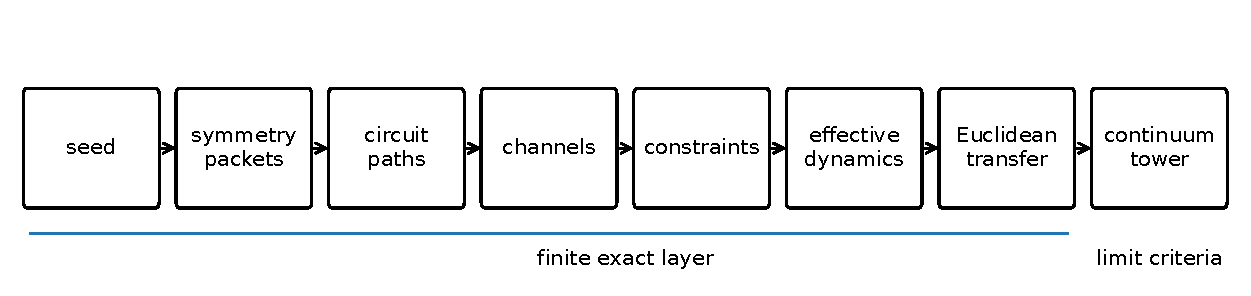
\includegraphics[width=\textwidth]{01_quantum_architecture.pdf}
\caption{The finite mathematical layers developed in the article and the separate limit criteria needed at the continuum boundary.}
\label{fig:architecture}
\end{figure}

\begin{table}[t]
\centering
\small
\begin{tabular}{>{\raggedright\arraybackslash}p{.20\textwidth}>{\raggedright\arraybackslash}p{.31\textwidth}>{\raggedright\arraybackslash}p{.39\textwidth}}
\toprule
Object & Packet coordinate & Exact structural condition \\
\midrule
State & \(P_a\psi\) & completeness of the projector family \\
Operator & \(P_bAP_a\) & block multiplication \\
Circuit & intermediate packet path & insertion of complete resolutions \\
Density matrix & \(P_a\rho P_b\) & two sided operator packets \\
Channel & superoperator block & complete positivity and covariance when declared \\
Code & syndrome packet & scalar compression of error products \\
Effective model & Feshbach map & invertibility of the hidden resolvent \\
Euclidean model & positive transfer matrix & positivity and self adjointness \\
Constraint system & quotient obstruction & commutator closure modulo the constraint span \\
Continuum tower & direct or norm limit & compatibility plus explicit convergence \\
\bottomrule
\end{tabular}
\caption{The packet coordinates used in the article.}
\label{tab:dictionary}
\end{table}

\section{Quantum seeds and observable algebras}\label{sec:seeds}

\begin{definition}[Finite quantum seed system]\label{def:quantum_seed}
A finite quantum seed system is a triple
\[
(\Hcal,\Acal,S),
\]
where \(\Hcal\) is a finite dimensional Hilbert space, \(\Acal\subseteq\End(\Hcal)\) is a unital star subalgebra, and \(S\subseteq\Hcal\) is a finite set. Its generated hull is
\[
\Acal S
=
\operatorname{span}\{A\psi:A\in\Acal,\ \psi\in S\}.
\]
The seed set is cyclic when \(\Acal S=\Hcal\). The quantum seed rank is the least cardinality of a cyclic seed set.
\end{definition}

The algebra is part of the data. A vector may be cyclic for \(\End(\Hcal)\) and fail to be cyclic for a restricted observable or gate algebra.

Let
\[
\Acal
\cong
\bigoplus_{r=1}^{s}
\bigl(M_{d_r}(\CC)\otimes I_{m_r}\bigr)
\]
act on
\[
\Hcal
\cong
\bigoplus_{r=1}^{s}
\bigl(\CC^{d_r}\otimes\CC^{m_r}\bigr).
\]
A vector in one block is identified with a \(d_r\) by \(m_r\) coefficient matrix.

\begin{theorem}[Orbit dimension of one seed]\label{thm:orbit_dimension}
For the action of \(M_d(\CC)\otimes I_m\) on \(\CC^d\otimes\CC^m\), let \(C_\psi\) be the coefficient matrix of \(\psi\). Then
\[
\dim\operatorname{span}\{(A\otimes I_m)\psi:A\in M_d(\CC)\}
=
 d\rank C_\psi.
\]
The vector is cyclic exactly when \(\rank C_\psi=m\).
\end{theorem}

\begin{proof}
Under the coefficient matrix identification, \((A\otimes I_m)\psi\) corresponds to \(AC_\psi\). Every row of \(AC_\psi\) lies in the row space of \(C_\psi\). Conversely, a matrix whose rows lie in that row space equals \(AC_\psi\) for a suitable \(A\). There are \(d\) independent row choices in a space of dimension \(\rank C_\psi\). The orbit dimension is therefore \(d\rank C_\psi\). It equals \(dm\) exactly when \(C_\psi\) has full column rank.
\end{proof}

\begin{theorem}[Quantum seed rank]\label{thm:quantum_seed_rank}
For the displayed multiplicity decomposition,
\[
\operatorname{srank}_{\Acal}(\Hcal)
=
\max_{1\le r\le s}
\left\lceil\frac{m_r}{d_r}\right\rceil.
\]
\end{theorem}

\begin{proof}
A single seed contributes a row space of dimension at most \(d_r\) to the \(r\)th multiplicity factor. Hence \(k\) seeds cover at most \(kd_r\) multiplicity directions, which gives the lower bound.

Set
\[
k=\max_r\left\lceil\frac{m_r}{d_r}\right\rceil.
\]
For each \(r\), partition a basis of \(\CC^{m_r}\) into at most \(k\) groups of size at most \(d_r\). Choose the coefficient matrix of the \(j\)th seed so that its row space spans the \(j\)th group. The combined row spaces span every multiplicity factor. The preceding theorem then shows that the \(k\) seeds generate every summand.
\end{proof}

\begin{corollary}[Local orbit and Schmidt rank]\label{cor:schmidt_orbit}
Let \(\psi\in\Hcal_A\otimes\Hcal_B\), let \(d_A=\dim\Hcal_A\), and let \(r\) be the Schmidt rank of \(\psi\). Then
\[
\dim\operatorname{span}\{(A\otimes I_B)\psi:A\in\End(\Hcal_A)\}
=
 d_A r.
\]
Local operators on \(A\) generate the whole bipartite Hilbert space exactly when the reduced state on \(B\) has full support.
\end{corollary}

\begin{proof}
The Schmidt rank is the rank of the coefficient matrix in any product basis. Apply \cref{thm:orbit_dimension}.
\end{proof}

\begin{figure}[t]
\centering
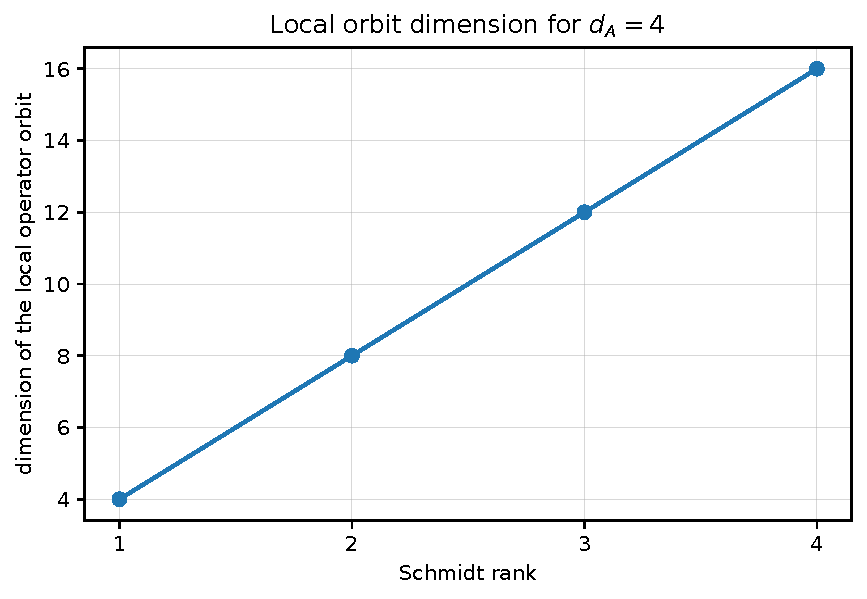
\includegraphics[width=.68\textwidth]{02_seed_rank.pdf}
\caption{The dimension reached by all local operators is linear in Schmidt rank.}
\label{fig:seed_rank}
\end{figure}

\begin{proposition}[Computational address orbit]\label{prop:computational_orbit}
For \(n\) qubits, let
\[
\psi_0=\ket{0}^{\otimes n}
\]
and let \(X_j\) be the Pauli \(X\) operator on the \(j\)th qubit. Then
\[
\left\{
X_1^{a_1}\cdots X_n^{a_n}\psi_0:
(a_1,\ldots,a_n)\in\{0,1\}^n
\right\}
\]
is the computational basis.
\end{proposition}

\begin{proof}
The addressed vector is \(\ket{a_1\cdots a_n}\). Distinct binary addresses produce the \(2^n\) distinct basis vectors.
\end{proof}

\begin{remark}\label{rem:seed_scope}
The seed rank records generation by a declared algebra. It does not measure circuit depth, locality cost, control complexity, or physical reachability under a restricted time dependent Hamiltonian.
\end{remark}

\section{Symmetry packets and selection rules}\label{sec:symmetry}

Let \(G\) be a finite group and let
\[
U:G\longrightarrow\Ucal(\Hcal)
\]
be a unitary representation. Write \(\widehat G\) for the set of irreducible unitary representations. For \(\lambda\in\widehat G\), let \(d_\lambda\) and \(\chi_\lambda\) denote its dimension and character.

\begin{theorem}[Finite group isotypic projectors]\label{thm:isotypic_projectors}
The operators
\[
P_\lambda
=
\frac{d_\lambda}{\abs{G}}
\sum_{g\in G}
\overline{\chi_\lambda(g)}U(g)
\]
are orthogonal projectors. They satisfy
\[
P_\lambda P_\mu=\delta_{\lambda\mu}P_\lambda,
\qquad
\sum_{\lambda\in\widehat G}P_\lambda=I_{\Hcal}.
\]
The range of \(P_\lambda\) is the \(\lambda\) isotypic component of \(\Hcal\).
\end{theorem}

\begin{proof}
Complete reducibility gives a unitary decomposition
\[
\Hcal
\cong
\bigoplus_{\mu\in\widehat G}
V_\mu\otimes M_\mu,
\qquad
U(g)
\cong
\bigoplus_\mu
\pi_\mu(g)\otimes I_{M_\mu}.
\]
On the \(\mu\) summand, the displayed average is central in the irreducible representation \(\pi_\mu\), so it is a scalar by Schur's lemma. Taking its trace and applying character orthogonality shows that the scalar is one when \(\mu=\lambda\) and zero otherwise. The asserted identities follow on the direct sum.
\end{proof}

The central projectors separate irreducible types but do not choose coordinates inside the representation factor. Matrix units provide that finer resolution.

\begin{theorem}[Representation matrix units]\label{thm:representation_matrix_units}
Fix an irreducible unitary representation \(\pi_\lambda:G\to U(d_\lambda)\) and an orthonormal basis of its representation space. Define
\[
E_{ij}^{\lambda}
=
\frac{d_\lambda}{\abs{G}}
\sum_{g\in G}
\bigl[\pi_\lambda(g^{-1})\bigr]_{ji}U(g).
\]
Then
\[
E_{ij}^{\lambda}E_{k\ell}^{\mu}
=
\delta_{\lambda\mu}\delta_{jk}E_{i\ell}^{\lambda},
\qquad
\bigl(E_{ij}^{\lambda}\bigr)^*=E_{ji}^{\lambda},
\]
and
\[
P_\lambda=\sum_{i=1}^{d_\lambda}E_{ii}^{\lambda}.
\]
\end{theorem}

\begin{proof}
Apply the matrix coefficient form of Schur orthogonality to the two group averages. It gives the matrix unit multiplication law. Unitarity gives the adjoint relation after replacing \(g\) by \(g^{-1}\). Summing the diagonal coefficients gives the character average in \cref{thm:isotypic_projectors}.
\end{proof}

\subsection{Cyclic charge packets}\label{subsec:cyclic_charge}

Let \(S\) be unitary with \(S^N=I\), and let \(\omega=\e^{2\pi\ii/N}\).

\begin{corollary}[Cyclic charge projectors]\label{cor:cyclic_projectors}
The operators
\[
P_j
=
\frac1N
\sum_{r=0}^{N-1}
\omega^{-jr}S^r,
\qquad
j\in\ZZ/N\ZZ,
\]
form a complete orthogonal packet system and satisfy
\[
SP_j=\omega^jP_j.
\]
\end{corollary}

\begin{proof}
Apply \cref{thm:isotypic_projectors} to the cyclic group. Its irreducible representations are the one dimensional characters \(r\mapsto\omega^{jr}\).
\end{proof}

\begin{definition}[Operator charge]\label{def:operator_charge}
An operator \(A\in\End(\Hcal)\) has cyclic charge \(q\in\ZZ/N\ZZ\) when
\[
SAS^*=\omega^qA.
\]
\end{definition}

\begin{theorem}[Charge selection rule]\label{thm:charge_selection}
If \(A\) has charge \(q\), then
\[
P_kAP_j=0
\]
unless \(k=j+q\) in \(\ZZ/N\ZZ\). In fact,
\[
AP_j=P_{j+q}AP_j.
\]
\end{theorem}

\begin{proof}
For \(x\in P_j\Hcal\),
\[
S(Ax)
=(SAS^*)Sx
=\omega^{q+j}Ax.
\]
Thus \(Ax\in P_{j+q}\Hcal\). The block statement follows.
\end{proof}

\begin{corollary}[Charge addition]\label{cor:charge_addition}
If \(A\) and \(B\) have charges \(q\) and \(r\), then \(AB\) has charge \(q+r\). The adjoint \(A^*\) has charge \(-q\).
\end{corollary}

\begin{proof}
Conjugation by \(S\) is a star automorphism. Apply it to \(AB\) and \(A^*\).
\end{proof}

\begin{figure}[t]
\centering
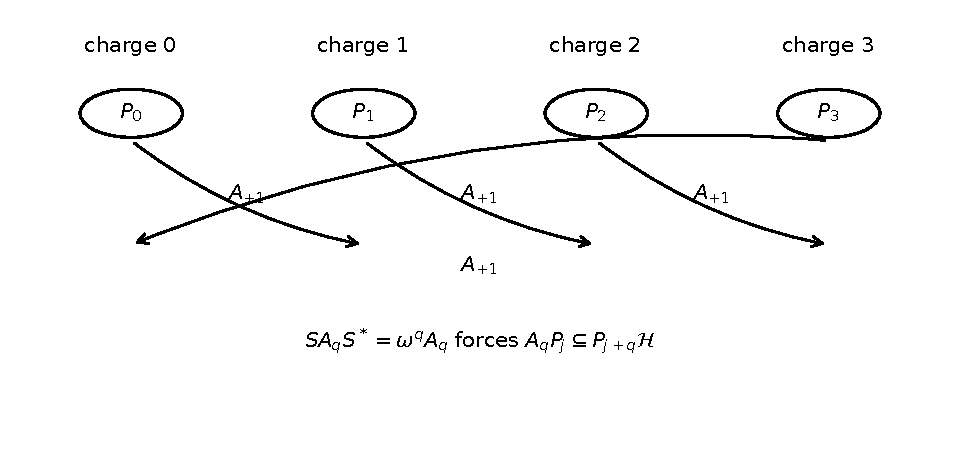
\includegraphics[width=.82\textwidth]{03_symmetry_selection.pdf}
\caption{A charge one operator moves each cyclic packet to the next packet and has no other transfer blocks.}
\label{fig:symmetry_selection}
\end{figure}

\subsection{Tensor refinement}\label{subsec:tensor_refinement}

Suppose the \(a\)th tensor factor carries a cyclic packet family
\[
\bigl(P_j^{(a)}\bigr)_{j\in\ZZ/N\ZZ}.
\]
The fine tensor packets are
\[
P_{\bm j}^{\rm fine}
=
P_{j_1}^{(1)}\otimes\cdots\otimes P_{j_m}^{(m)}.
\]

\begin{theorem}[Tensor charge refinement]\label{thm:tensor_refinement}
For \(r\in\ZZ/N\ZZ\), define
\[
P_r^{\rm total}
=
\sum_{j_1+\cdots+j_m=r}
P_{j_1}^{(1)}\otimes\cdots\otimes P_{j_m}^{(m)}.
\]
Then the \(P_r^{\rm total}\) form a complete orthogonal packet system. Every total charge packet is the exact sum of its fine tensor descendants.
\end{theorem}

\begin{proof}
The fine tensor projectors are mutually orthogonal and sum to the identity. The total residue classes partition the fine address set. Summing the fine projectors over each class gives the result.
\end{proof}

\begin{corollary}[Tensor selection rule]\label{cor:tensor_selection}
If \(A_a\) has local charge \(q_a\), then
\[
A_1\otimes\cdots\otimes A_m
\]
has total charge \(q_1+\cdots+q_m\).
\end{corollary}

\begin{proof}
Conjugate the tensor product by the total cyclic symmetry and multiply the local phase factors.
\end{proof}

\begin{remark}\label{rem:nonabelian_fusion}
For a nonabelian group, tensor products are refined by irreducible fusion multiplicities rather than residue addition. The central isotypic projectors remain exact, but a complete tensor refinement also requires a choice of Clebsch Gordan intertwiners.
\end{remark}

\section{Quantum circuits as packet paths}\label{sec:circuits}

Let
\[
U=U_mU_{m-1}\cdots U_1
\]
be a finite circuit and let \((P_a)_{a\in I}\) be a complete orthogonal packet family.

\begin{theorem}[Exact circuit path expansion]\label{thm:circuit_path}
For source packet \(a_0\) and target packet \(a_m\),
\[
P_{a_m}UP_{a_0}
=
\sum_{a_1,\ldots,a_{m-1}}
P_{a_m}U_mP_{a_{m-1}}
\cdots
P_{a_1}U_1P_{a_0}.
\]
Summing over \(a_0\) and \(a_m\) reconstructs \(U\).
\end{theorem}

\begin{proof}
Insert \(I=\sum_aP_a\) between every adjacent pair of gates and distribute the finite sums. Completeness at the two endpoints gives the full operator.
\end{proof}

For a packet path
\[
\gamma=(a_0,a_1,\ldots,a_m),
\]
write
\[
U_\gamma
=
P_{a_m}U_mP_{a_{m-1}}
\cdots
P_{a_1}U_1P_{a_0}.
\]

\begin{theorem}[Packet unitarity identities]\label{thm:packet_unitarity}
If \(U\) is unitary and \(U_{ba}=P_bUP_a\), then
\[
\sum_bU_{ba}^*U_{bc}=\delta_{ac}P_a
\]
and
\[
\sum_aU_{ba}U_{da}^*=\delta_{bd}P_b.
\]
\end{theorem}

\begin{proof}
Use completeness and unitarity:
\[
\sum_bU_{ba}^*U_{bc}
=
P_aU^*\left(\sum_bP_b\right)UP_c
=P_aP_c.
\]
The second identity follows in the same way.
\end{proof}

\begin{corollary}[Probability conservation from one packet]\label{cor:packet_probability}
If \(\psi\in P_a\Hcal\), then
\[
\sum_b\norm{P_bU\psi}^2=\norm{\psi}^2.
\]
\end{corollary}

\begin{proof}
Take the inner product of the first identity in \cref{thm:packet_unitarity} with \(\psi\) and set \(c=a\).
\end{proof}

\begin{theorem}[Path interference formula]\label{thm:path_interference}
Fix a source vector \(\psi\in P_{a_0}\Hcal\) and a target packet \(b\). Let \(\Gamma_b\) be the set of packet paths from \(a_0\) to \(b\), and set
\[
\eta_\gamma=U_\gamma\psi.
\]
Then
\[
\norm{P_bU\psi}^2
=
\sum_{\gamma\in\Gamma_b}\norm{\eta_\gamma}^2
+
2\operatorname{Re}
\sum_{\substack{\gamma,\gamma'\in\Gamma_b\\ \gamma<\gamma'}}
\ip{\eta_\gamma}{\eta_{\gamma'}}.
\]
Consequently,
\[
\norm{P_bU\psi}
\leq
\sum_{\gamma\in\Gamma_b}\norm{\eta_\gamma}.
\]
If the path outputs are pairwise orthogonal, the target probability is the sum of the path probabilities.
\end{theorem}

\begin{proof}
The path expansion gives
\[
P_bU\psi=\sum_{\gamma\in\Gamma_b}\eta_\gamma.
\]
Expand the squared norm and group conjugate cross terms. The norm bound is the triangle inequality. Orthogonality removes every cross term.
\end{proof}

\begin{proposition}[Charge pruning of circuit paths]\label{prop:charge_pruning}
Suppose every gate has a finite charge decomposition
\[
U_r=\sum_qU_r^{(q)},
\qquad
SU_r^{(q)}S^*=\omega^qU_r^{(q)}.
\]
A term with gate charges \(q_1,\ldots,q_m\) can contribute from source charge \(a_0\) only to target charge
\[
a_m=a_0+q_1+\cdots+q_m.
\]
Every packet path violating one of the intermediate charge updates vanishes.
\end{proposition}

\begin{proof}
Apply \cref{thm:charge_selection} after each gate component. The packet address is forced at every step.
\end{proof}

\begin{figure}[t]
\centering
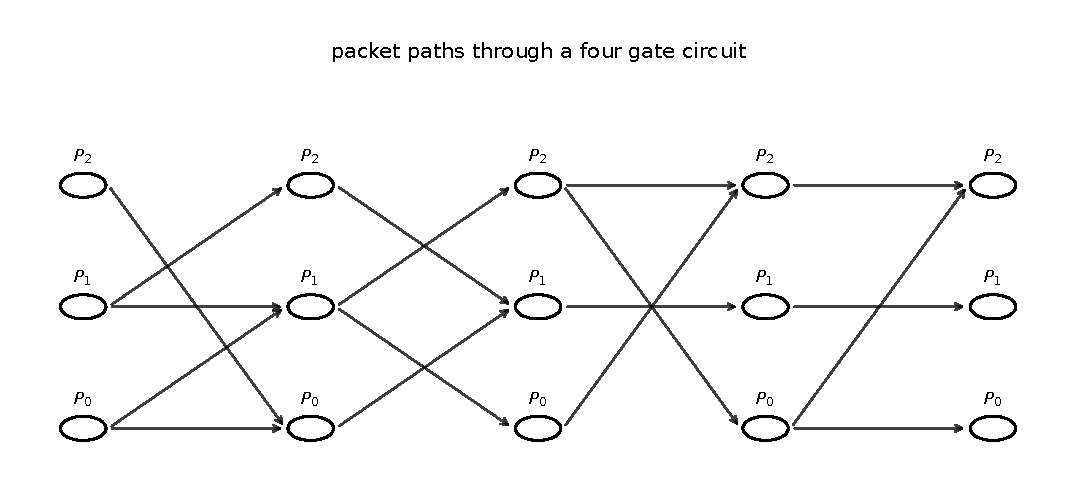
\includegraphics[width=.88\textwidth]{04_circuit_paths.pdf}
\caption{A circuit block is the coherent sum of its allowed packet paths. Selection rules remove forbidden paths before amplitudes are evaluated.}
\label{fig:circuit_paths}
\end{figure}

\begin{example}[Bell circuit]\label{ex:bell_circuit}
Starting from \(\ket{00}\), apply a Hadamard gate to the first qubit and then a controlled not gate. The final state is
\[
\frac{\ket{00}+\ket{11}}{\sqrt2}.
\]
It lies in the even parity packet. The intermediate state has one even and one odd computational contribution, so the final even amplitude is reconstructed by more than one packet path.
\end{example}

\section{Symmetry resolved dynamics and leakage}\label{sec:dynamics}

Let \(H=H^*\) and let \((P_a)_{a\in I}\) be a complete orthogonal packet system.

\begin{theorem}[Exact invariant packets]\label{thm:invariant_packets}
The following conditions are equivalent:
\begin{enumerate}
\item \([H,P_a]=0\) for every \(a\)
\item \(P_bHP_a=0\) whenever \(a\neq b\)
\item every packet \(P_a\Hcal\) is invariant under \(\e^{-\ii tH}\) for every real \(t\)
\end{enumerate}
When they hold,
\[
H=\sum_aP_aHP_a
\]
and
\[
\e^{-\ii tH}=\sum_aP_a\e^{-\ii tH}P_a.
\]
\end{theorem}

\begin{proof}
Commutation is equivalent to vanishing of every off diagonal block. The same block decomposition passes to polynomials in \(H\), then to the exponential by norm convergence. Invariance of every packet implies invariance under both \(\e^{-\ii tH}\) and its adjoint. Differentiation at \(t=0\) gives commutation with \(H\).
\end{proof}

Fix one packet projector \(P\) and set \(Q=I-P\).

\begin{lemma}[Off diagonal norm]\label{lem:off_diagonal_norm}
For self adjoint \(H\),
\[
\norm{[H,P]}=\norm{QHP}=\norm{PHQ}.
\]
\end{lemma}

\begin{proof}
Relative to \(P\Hcal\oplus Q\Hcal\),
\[
[H,P]
=
\begin{pmatrix}
0&-PHQ\\
QHP&0
\end{pmatrix}.
\]
Its square has diagonal blocks \(-PHQHP\) and \(-QHPHQ\). The norm is therefore the largest singular value of \(QHP\).
\end{proof}

\begin{theorem}[Fixed packet leakage]\label{thm:fixed_leakage}
For every real \(t\),
\[
\norm{Q\e^{-\ii tH}P}
\leq
\abs{t}\norm{QHP}
=
\abs{t}\norm{[H,P]}.
\]
\end{theorem}

\begin{proof}
Let
\[
H_{\rm d}=PHP+QHQ,
\qquad
H_{\rm o}=PHQ+QHP.
\]
The propagator generated by \(H_{\rm d}\) preserves \(P\Hcal\) and \(Q\Hcal\). Duhamel's formula relative to \(H_{\rm d}\) gives
\[
Q\e^{-\ii tH}P
=
-\ii
\int_0^t
Q\e^{-\ii(t-s)H}H_{\rm o}\e^{-\ii sH_{\rm d}}P
\dd s.
\]
Since \(H_{\rm o}P=QHP\) and both propagators are unitary, the norm is at most \(\abs{t}\norm{QHP}\). Use \cref{lem:off_diagonal_norm} for the last equality.
\end{proof}

\begin{figure}[t]
\centering
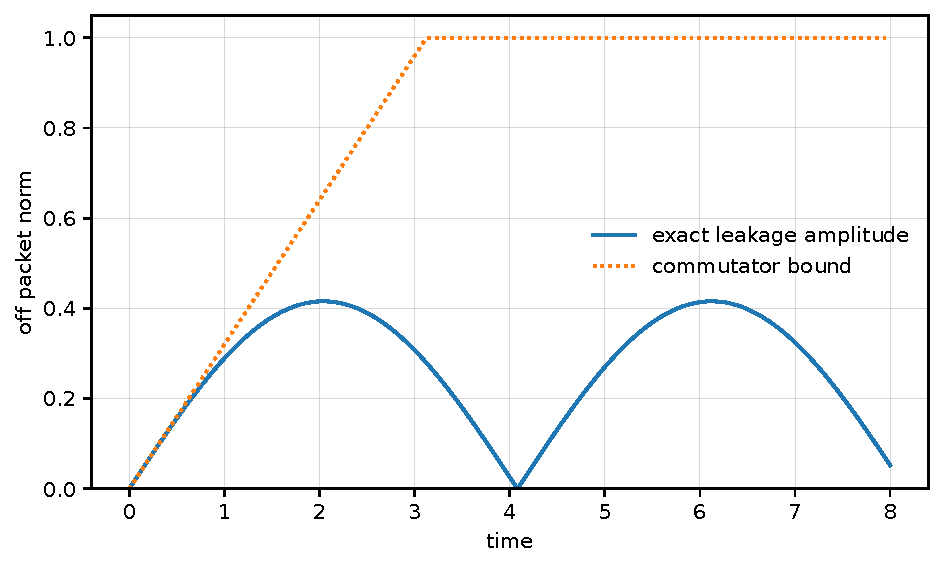
\includegraphics[width=.72\textwidth]{05_leakage_bound.pdf}
\caption{Exact transition amplitude in a two packet model and the linear commutator bound.}
\label{fig:leakage}
\end{figure}

\begin{corollary}[Leakage probability]\label{cor:leakage_probability}
If \(\psi\in P\Hcal\) is a unit vector, then
\[
\norm{Q\e^{-\ii tH}\psi}^2
\leq
 t^2\norm{QHP}^2.
\]
\end{corollary}

\begin{proof}
Apply \cref{thm:fixed_leakage} and square the result.
\end{proof}

\section{Moving packets and geometric transport}\label{sec:moving_packets}

Let \((P_a(t))_{a\in I}\) be a twice continuously differentiable family of complete orthogonal packet systems on a finite dimensional Hilbert space.

\begin{theorem}[Canonical packet connection]\label{thm:kato_connection}
Define
\[
K(t)
=
\sum_a\dot P_a(t)P_a(t).
\]
Then
\[
K(t)^*=-K(t)
\]
and
\[
[K(t),P_a(t)]=\dot P_a(t)
\]
for every \(a\).
\end{theorem}

\begin{proof}
Differentiating \(P_a^2=P_a\) gives
\[
\dot P_aP_a+P_a\dot P_a=\dot P_a.
\]
Summing over \(a\) and using \(\sum_a\dot P_a=0\) yields
\[
\sum_aP_a\dot P_a=-\sum_a\dot P_aP_a.
\]
This proves skew adjointness. For fixed \(b\),
\[
KP_b=\dot P_bP_b.
\]
Differentiating \(P_bP_a=0\) for \(a\neq b\) gives
\[
P_b\dot P_a=-\dot P_bP_a.
\]
Hence
\[
P_bK=-\dot P_b(I-P_b).
\]
Subtracting gives \([K,P_b]=\dot P_b\).
\end{proof}

\begin{theorem}[Exact Kato transport]\label{thm:kato_transport}
Let \(W(t)\) solve
\[
\dot W(t)=K(t)W(t),
\qquad
W(0)=I.
\]
Then \(W(t)\) is unitary and
\[
P_a(t)W(t)=W(t)P_a(0)
\]
for every packet \(a\).
\end{theorem}

\begin{proof}
Skew adjointness gives
\[
\frac{\dd}{\dd t}W(t)^*W(t)=0.
\]
Thus \(W(t)\) is unitary. Next,
\[
\frac{\dd}{\dd t}
\left(W(t)^*P_a(t)W(t)\right)
=
W(t)^*
\left(
\dot P_a-[K,P_a]
\right)
W(t)=0.
\]
The expression equals \(P_a(0)\) at \(t=0\), which proves the intertwining identity.
\end{proof}

\begin{theorem}[Moving frame Hamiltonian]\label{thm:moving_frame}
Let \(U(t)\) solve
\[
\ii\dot U(t)=H(t)U(t),
\qquad
U(0)=I,
\]
where \(H(t)=H(t)^*\). Set
\[
V(t)=W(t)^*U(t).
\]
Then
\[
\ii\dot V(t)=H_{\rm mov}(t)V(t),
\]
where
\[
H_{\rm mov}(t)
=
W(t)^*H(t)W(t)-\ii W(t)^*\dot W(t)
=
W(t)^*\bigl(H(t)-\ii K(t)\bigr)W(t).
\]
The moving frame Hamiltonian is self adjoint.
\end{theorem}

\begin{proof}
Differentiate \(V=W^*U\). Since \(\dot W=KW\) and \(K^*=-K\),
\[
\dot W^*=-W^*K.
\]
Substitution gives the equation. The first term in \(H_{\rm mov}\) is self adjoint. The operator \(-\ii W^*\dot W\) is self adjoint because \(W^*\dot W\) is skew adjoint.
\end{proof}

\begin{theorem}[Moving packet leakage]\label{thm:moving_leakage}
Fix a packet \(P(t)=P_a(t)\) and put \(Q(t)=I-P(t)\). For \(0\leq t\leq T\),
\[
\norm{Q(t)U(t)P(0)}
\leq
\int_0^t
\norm{Q(s)\bigl(H(s)-\ii K(s)\bigr)P(s)}
\dd s.
\]
In particular, the physical evolution follows the moving packet exactly on \([0,T]\) when the displayed off packet block vanishes for every time in that interval.
\end{theorem}

\begin{proof}
In the Kato frame, \(P(0)\) is fixed and
\[
Q(t)U(t)P(0)
=
W(t)Q(0)V(t)P(0).
\]
Apply the time dependent version of the Duhamel argument in \cref{thm:fixed_leakage} to \(H_{\rm mov}(t)\). The off diagonal block is
\[
Q(0)H_{\rm mov}(s)P(0)
=
W(s)^*Q(s)\bigl(H(s)-\ii K(s)\bigr)P(s)W(s).
\]
Unitary conjugation preserves the norm.
\end{proof}

The geometric term is therefore part of the exact coupling test. A Hamiltonian may be packet diagonal at every fixed time and still fail to transport the moving packet because the packet itself rotates.

\subsection{Discrete packet transport}\label{subsec:discrete_transport}

Let \((P_a)\) and \((Q_a)\) be two complete packet systems with the same index set. Define
\[
S(\Qcal,\Pcal)=\sum_aQ_aP_a.
\]

\begin{theorem}[Direct packet rotation]\label{thm:direct_rotation}
Assume
\[
\norm{S(\Qcal,\Pcal)-I}<1.
\]
Then \(S(\Qcal,\Pcal)\) is invertible. Its unitary polar factor
\[
\Ucal(\Qcal,\Pcal)
=
S(S^*S)^{-1/2}
\]
satisfies
\[
Q_a\Ucal(\Qcal,\Pcal)
=
\Ucal(\Qcal,\Pcal)P_a
\]
for every \(a\).
\end{theorem}

\begin{proof}
The norm condition gives invertibility by the Neumann series. The identity
\[
Q_aS=SP_a=Q_aP_a
\]
shows that \(S^*S\) commutes with every \(P_a\). Its inverse square root also commutes with every \(P_a\). Hence
\[
Q_a\Ucal
=Q_aS(S^*S)^{-1/2}
=SP_a(S^*S)^{-1/2}
=\Ucal P_a.
\]
The polar factor is unitary because \(S\) is invertible.
\end{proof}

\begin{theorem}[Convergence of short packet rotations]\label{thm:short_rotation_convergence}
Let \((P_a(t))\) be twice continuously differentiable on \([0,T]\). For a partition
\[
0=t_0<t_1<\cdots<t_n=T,
\]
let
\[
W_\pi
=
\Ucal\bigl(\Pcal(t_n),\Pcal(t_{n-1})\bigr)
\cdots
\Ucal\bigl(\Pcal(t_1),\Pcal(t_0)\bigr).
\]
For sufficiently fine partitions the factors are defined, and
\[
\norm{W_\pi-W(T)}
\leq
C_T\abs{\pi}
\]
for a constant depending on the packet path but not on the partition.
\end{theorem}

\begin{proof}
Taylor expansion gives
\[
S\bigl(\Pcal(t+h),\Pcal(t)\bigr)
=
I+hK(t)+O(h^2)
\]
uniformly on \([0,T]\). Since \(K(t)^*=-K(t)\),
\[
S^*S=I+O(h^2),
\]
so the polar factor satisfies
\[
\Ucal\bigl(\Pcal(t+h),\Pcal(t)\bigr)
=
I+hK(t)+O(h^2).
\]
This is a first order one step approximation to \(\dot W=KW\). A telescoping product estimate over the partition gives a total error bounded by a constant times \(\sum_j(t_{j+1}-t_j)^2\), which is at most \(T\abs{\pi}\).
\end{proof}

\begin{figure}[t]
\centering
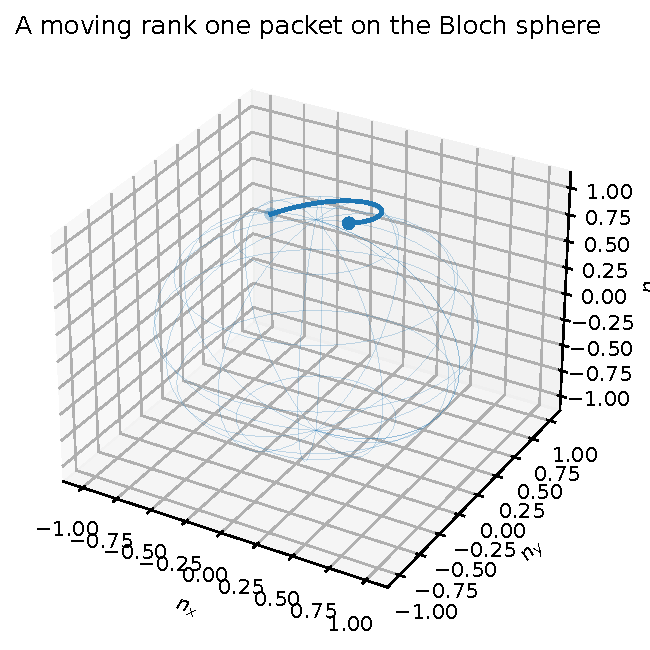
\includegraphics[width=.62\textwidth]{06_kato_transport.pdf}
\caption{A moving rank one packet on the Bloch sphere. The Kato evolution transports the range without choosing a phase convention for its eigenvector.}
\label{fig:kato_transport}
\end{figure}

\subsection{Local frames and curvature}\label{subsec:curvature}

Let \(P(x)\) be a smooth rank \(r\) orthogonal projector over a parameter manifold. Choose a local isometry
\[
V(x):\CC^r\longrightarrow\Hcal,
\qquad
V(x)V(x)^*=P(x).
\]

\begin{theorem}[Nonabelian packet connection]\label{thm:nonabelian_connection}
The matrix valued one form
\[
\Acal=V^*\dd V
\]
is skew adjoint. Under a frame change \(V'=VG\), where \(G(x)\in U(r)\),
\[
\Acal'
=
G^*\Acal G+G^*\dd G.
\]
Its curvature
\[
\Fcal=\dd\Acal+\Acal\wedge\Acal
\]
satisfies
\[
\Fcal=V^*(\dd P\wedge\dd P)V.
\]
\end{theorem}

\begin{proof}
Differentiate \(V^*V=I\) to obtain \(\Acal^*=-\Acal\). The gauge transformation law follows by differentiating \(VG\). Since \(P=VV^*\) and \((I-P)\dd V=\dd P\,V\), direct expansion gives
\[
\dd\Acal+\Acal\wedge\Acal
=
\dd V^*(I-P)\wedge\dd V
=
V^*(\dd P\wedge\dd P)V.
\]
\end{proof}

\begin{corollary}[Bloch sphere curvature]\label{cor:bloch_curvature}
Let
\[
P(\theta,\phi)
=
\frac12\left(I+\bm n(\theta,\phi)\cdot\bm\sigma\right),
\]
where
\[
\bm n=(\sin\theta\cos\phi,\sin\theta\sin\phi,\cos\theta).
\]
With the convention
\[
\Fcal_{\theta\phi}
=-\ii\Tr\bigl(P[\partial_\theta P,\partial_\phi P]\bigr),
\]
one has
\[
\Fcal_{\theta\phi}=\frac12\sin\theta
\]
and
\[
\frac1{2\pi}
\int_0^{2\pi}\int_0^\pi
\Fcal_{\theta\phi}\dd\theta\dd\phi
=1.
\]
\end{corollary}

\begin{proof}
The Pauli identity
\[
(\bm a\cdot\bm\sigma)(\bm b\cdot\bm\sigma)
=(\bm a\cdot\bm b)I
+\ii(\bm a\times\bm b)\cdot\bm\sigma
\]
gives
\[
-\ii\Tr\bigl(P[\partial_\theta P,\partial_\phi P]\bigr)
=\frac12
\bm n\cdot
(\partial_\theta\bm n\times\partial_\phi\bm n)
=\frac12\sin\theta.
\]
Integration gives one.
\end{proof}

\section{Operator packets, measurements, and quantum channels}\label{sec:channels}

Density matrices and observables carry both an input packet and an output packet. Equip \(\End(\Hcal)\) with the Hilbert Schmidt inner product
\[
\ip{X}{Y}_{\HS}=\Tr(X^*Y).
\]

\begin{definition}[Two sided operator packet]\label{def:operator_packet}
For a complete orthogonal family \((P_a)\), define
\[
\Pcal_{ab}(X)=P_aXP_b.
\]
The range
\[
\Bcal_{ab}=P_a\End(\Hcal)P_b
\]
is the operator packet with output address \(a\) and input address \(b\).
\end{definition}

\begin{theorem}[Complete operator packet system]\label{thm:operator_packets}
The superoperators \((\Pcal_{ab})_{a,b\in I}\) are mutually orthogonal projections on Hilbert Schmidt operator space. They satisfy
\[
X=\sum_{a,b}P_aXP_b
\]
and
\[
\norm{X}_{\HS}^2
=
\sum_{a,b}\norm{P_aXP_b}_{\HS}^2.
\]
\end{theorem}

\begin{proof}
Idempotence and completeness follow from the projector identities. For Hilbert Schmidt orthogonality,
\[
\begin{aligned}
\ip{P_aXP_b}{P_cYP_d}_{\HS}
&=
\Tr(P_bX^*P_aP_cYP_d)\\
&=
\delta_{ac}\delta_{bd}
\Tr(P_bX^*P_aYP_b).
\end{aligned}
\]
The Pythagorean identity follows.
\end{proof}

\begin{figure}[t]
\centering
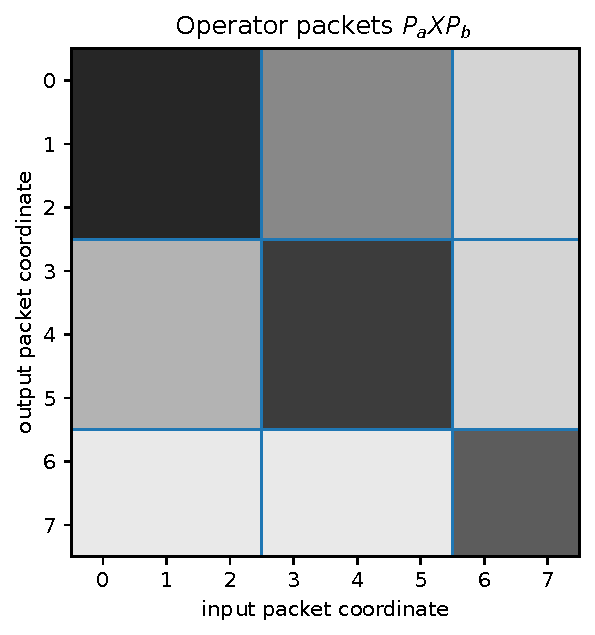
\includegraphics[width=.58\textwidth]{07_operator_packets.pdf}
\caption{A density matrix or observable carries two packet addresses. Diagonal packets contain populations and internal observables. Off diagonal packets contain coherences.}
\label{fig:operator_packets}
\end{figure}

\begin{definition}[Packet dephasing]\label{def:dephasing}
The packet dephasing map is
\[
\Dcal_{\Pcal}(X)=\sum_aP_aXP_a.
\]
\end{definition}

\begin{theorem}[Dephasing as conditional expectation]\label{thm:dephasing_expectation}
The map \(\Dcal_{\Pcal}\) is completely positive, trace preserving, unital, and idempotent. It is the Hilbert Schmidt orthogonal projection onto the block diagonal algebra
\[
\Acal_{\Pcal}
=
\{X:[X,P_a]=0\text{ for every }a\}.
\]
In particular,
\[
\norm{\Dcal_{\Pcal}(X)}_{\HS}
\leq
\norm{X}_{\HS}.
\]
\end{theorem}

\begin{proof}
The projectors \(P_a\) form a Kraus family because \(\sum_aP_a^*P_a=I\). Thus the map is completely positive and trace preserving. It is unital for the same reason. Orthogonality and idempotence follow from \cref{thm:operator_packets}. Its range consists exactly of the diagonal operator packets, which is the commutant of the projector family.
\end{proof}

\begin{corollary}[Block diagonal measurement invariance]\label{cor:measurement_invariance}
Let \((E_k)\) be a positive operator valued measurement, and suppose
\[
E_k=\Dcal_{\Pcal}(E_k)
\]
for every \(k\). Then every density matrix \(\rho\) satisfies
\[
\Tr(E_k\rho)
=
\Tr\bigl(E_k\Dcal_{\Pcal}(\rho)\bigr).
\]
\end{corollary}

\begin{proof}
Since \(\Dcal_{\Pcal}\) is self adjoint for the Hilbert Schmidt inner product,
\[
\Tr(E_k\rho)
=
\Tr\bigl(\Dcal_{\Pcal}(E_k)\rho\bigr)
=
\Tr\bigl(E_k\Dcal_{\Pcal}(\rho)\bigr).
\]
\end{proof}

\subsection{Channel superblocks}\label{subsec:channel_blocks}

Let \(\Phi:\End(\Hcal_X)\to\End(\Hcal_Y)\) be linear. Choose packet systems \((P_a)\) on \(\Hcal_X\) and \((Q_c)\) on \(\Hcal_Y\). Define
\[
\Phi_{cd,ab}
=
\Qcal_{cd}\Phi\Pcal_{ab}.
\]

\begin{theorem}[Exact channel block calculus]\label{thm:channel_blocks}
Every linear map has the exact reconstruction
\[
\Phi=\sum_{a,b,c,d}\Phi_{cd,ab}.
\]
If \(\Psi:\End(\Hcal_Y)\to\End(\Hcal_Z)\), then
\[
(\Psi\Phi)_{ef,ab}
=
\sum_{c,d}
\Psi_{ef,cd}\Phi_{cd,ab}.
\]
\end{theorem}

\begin{proof}
Insert the complete operator packet resolutions before and after \(\Phi\). For composition, insert the middle resolution between \(\Psi\) and \(\Phi\) and collect the output and input packets.
\end{proof}

\begin{standardfact}[Finite Kraus and Choi criteria]\label{fact:kraus_choi}
A linear map \(\Phi:M_n(\CC)\to M_m(\CC)\) is completely positive exactly when it has a Kraus representation
\[
\Phi(X)=\sum_rK_rXK_r^*.
\]
It is trace preserving exactly when
\[
\sum_rK_r^*K_r=I.
\]
Equivalently, its Choi matrix
\[
J(\Phi)
=
\sum_{i,j}\Phi(\ket{i}\bra{j})\otimes\ket{i}\bra{j}
\]
is positive, and trace preservation is
\[
\Tr_{\rm out}J(\Phi)=I_{\rm in}.
\]
\end{standardfact}

These finite criteria are classical \cite{Stinespring1955,Choi1975,Kraus1983,Watrous2018}.

\subsection{Covariance and coherence order}\label{subsec:channel_covariance}

Let \(S^N=I\) and define the conjugation action
\[
\Ad_S(X)=SXS^*.
\]

\begin{theorem}[Coherence order projectors]\label{thm:coherence_projectors}
For \(q\in\ZZ/N\ZZ\), define
\[
\Lcal_q(X)
=
\frac1N
\sum_{r=0}^{N-1}
\omega^{-qr}S^rXS^{-r}.
\]
Then the \(\Lcal_q\) form a complete orthogonal packet system on Hilbert Schmidt operator space. Their ranges are the operators satisfying
\[
SXS^*=\omega^qX.
\]
If \(P_j\) are the state charge projectors, then
\[
\Ran\Lcal_q
=
\bigoplus_jP_{j+q}\End(\Hcal)P_j.
\]
\end{theorem}

\begin{proof}
Apply the cyclic character projector formula to the unitary representation \(\Ad_S\) on operator space. The last identity follows from \cref{thm:charge_selection} applied to each operator packet.
\end{proof}

\begin{theorem}[Covariant channels preserve coherence order]\label{thm:covariant_channel}
Suppose
\[
\Phi(SXS^*)=S\Phi(X)S^*
\]
for every \(X\). Then
\[
\Phi\Lcal_q=\Lcal_q\Phi
\]
for every \(q\). Thus \(\Phi\) cannot mix distinct coherence orders.
\end{theorem}

\begin{proof}
The covariance identity says that \(\Phi\) commutes with every power of \(\Ad_S\). It therefore commutes with each finite character average \(\Lcal_q\).
\end{proof}

\begin{theorem}[Choi symmetry criterion]\label{thm:choi_covariance}
Let \(U:G\to\Ucal(\Hcal)\) be a finite group representation. A channel \(\Phi\) is covariant,
\[
\Phi\bigl(U(g)XU(g)^*\bigr)
=
U(g)\Phi(X)U(g)^*,
\]
if and only if
\[
\bigl(U(g)\otimes\overline{U(g)}\bigr)
J(\Phi)
\bigl(U(g)^*\otimes U(g)^{\mathsf T}\bigr)
=
J(\Phi)
\]
for every \(g\in G\).
\end{theorem}

\begin{proof}
Let
\[
\Omega=\sum_i\ket{i}\otimes\ket{i}.
\]
Then
\[
J(\Phi)=(\Phi\otimes\id)(\ket{\Omega}\bra{\Omega}).
\]
The vector \(\Omega\) is invariant under \(U\otimes\overline U\). Covariance therefore implies the displayed Choi invariance. Conversely, the displayed transformation is the Choi matrix of
\[
\Ad_{U(g)}\circ\Phi\circ\Ad_{U(g)^*}.
\]
The Choi correspondence is injective, so invariance implies that this map equals \(\Phi\), which is covariance.
\end{proof}

\begin{corollary}[Choi packet decomposition]\label{cor:choi_packets}
The Choi matrix of a covariant channel is block diagonal with respect to the isotypic decomposition of \(U\otimes\overline U\).
\end{corollary}

\begin{proof}
Apply \cref{thm:isotypic_projectors} to the representation \(U\otimes\overline U\) and use \cref{thm:choi_covariance}.
\end{proof}

\begin{example}[Amplitude damping]\label{ex:amplitude_damping}
For \(0\leq\gamma\leq1\), let
\[
K_0=
\begin{pmatrix}
1&0\\
0&\sqrt{1-\gamma}
\end{pmatrix},
\qquad
K_1=
\begin{pmatrix}
0&\sqrt\gamma\\
0&0
\end{pmatrix}.
\]
The channel
\[
\Phi_\gamma(\rho)=K_0\rho K_0^*+K_1\rho K_1^*
\]
is trace preserving. It sends the off diagonal packet \(\ket0\bra1\) to \(\sqrt{1-\gamma}\ket0\bra1\), while the excited population transfers partly into the ground population.
\end{example}

\begin{figure}[t]
\centering
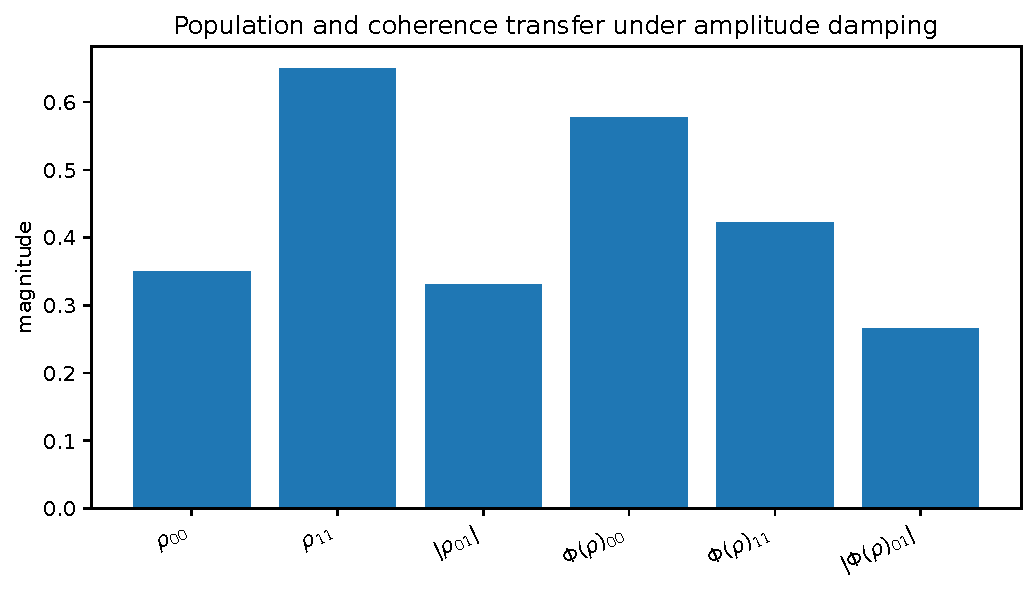
\includegraphics[width=.82\textwidth]{08_channel_coherence.pdf}
\caption{Amplitude damping transfers population and contracts the coherence packet.}
\label{fig:channel_coherence}
\end{figure}


\subsection{Quantum dynamical semigroups}\label{subsec:lindblad}

\begin{standardfact}[Finite Lindblad generator]\label{fact:lindblad}
A norm continuous quantum dynamical semigroup on a finite matrix algebra has a generator of the form
\[
\Gcal(X)
=
-\ii[H,X]
+
\sum_r
\left(
L_rXL_r^*
-
\frac12L_r^*L_rX
-
\frac12XL_r^*L_r
\right),
\]
where \(H=H^*\). Conversely, every operator of this form generates a completely positive trace preserving semigroup \cite{Lindblad1976}.
\end{standardfact}

\begin{theorem}[Charge preservation by a Lindblad generator]\label{thm:lindblad_charge}
Let \(S^N=I\). Assume
\[
SHS^*=H
\]
and, for every jump operator, there is a charge \(q_r\) such that
\[
SL_rS^*=\omega^{q_r}L_r.
\]
Then the Lindblad generator \(\Gcal\) preserves every coherence order:
\[
\Gcal\Lcal_p=\Lcal_p\Gcal.
\]
The quantum dynamical semigroup \(\e^{t\Gcal}\) has the same property.
\end{theorem}

\begin{proof}
Let \(X\) have coherence order \(p\). The Hamiltonian commutator has order \(p\) because \(H\) has charge zero. The jump term \(L_rXL_r^*\) has charge
\[
q_r+p-q_r=p.
\]
Also \(L_r^*L_r\) has charge zero, so both anticommutator terms have charge \(p\). Thus \(\Gcal\) preserves \(\Ran\Lcal_p\). The exponential series then shows that \(\e^{t\Gcal}\) preserves the same packets.
\end{proof}

\begin{corollary}[Independent coherence evolution]\label{cor:no_coherence_mixing}
Under the hypotheses of \cref{thm:lindblad_charge}, each coherence component of an initial operator evolves within its own order. In particular, a density matrix in the zero order sector remains in that sector.
\end{corollary}

\begin{proof}
Decompose the initial operator by \cref{thm:coherence_projectors} and apply the invariant packet statement to each component.
\end{proof}

The theorem does not say that every diagonal quantum master equation closes to a classical Markov chain on packet populations. Scalar population closure needs additional isotropy inside each packet.

\section{Quantum error correction as a compression obstruction}\label{sec:qec}

Let \(P\) be the orthogonal projector onto a code space
\[
\Ccal=P\Hcal,
\qquad
k=\dim\Ccal.
\]
The compression of \(A\in\End(\Hcal)\) to the code is \(PAP\in\End(\Ccal)\).

\begin{definition}[Code compression obstruction]\label{def:code_obstruction}
Let
\[
q_P:\End(\Ccal)\longrightarrow\End(\Ccal)/(\CC I_{\Ccal})
\]
be the quotient map. Define
\[
\Ob_P(A)=q_P(PAP).
\]
Equivalently, one may use the traceless representative
\[
\ob_P(A)
=
PAP-
\frac{\Tr(PAP)}{k}P.
\]
\end{definition}

The class vanishes exactly when \(A\) acts as a scalar after compression to the code. Such an operator cannot distinguish normalized code vectors by expectation value.

\begin{theorem}[Knill Laflamme as obstruction vanishing]\label{thm:kl_obstruction}
Let \(E_1,\ldots,E_r\) be an error family. The code \(\Ccal\) corrects their linear span exactly if and only if
\[
\Ob_P(E_a^*E_b)=0
\]
for all \(a,b\). Equivalently, there is a matrix \(c=(c_{ab})\) such that
\[
PE_a^*E_bP=c_{ab}P
\]
for all \(a,b\).
\end{theorem}

\begin{proof}
The equivalence between the quotient statement and the scalar compression identity is immediate from the definition. The latter identity is the finite Knill Laflamme criterion \cite{KnillLaflamme1997,SchumacherNielsen1996}.
\end{proof}

The next result gives the packet construction behind the criterion.

\begin{theorem}[Orthogonal syndrome construction]\label{thm:syndrome_construction}
Assume the Knill Laflamme identities. Then the coefficient matrix \(c\) is positive semidefinite. Choose a unitary matrix \(W\) such that
\[
WcW^*=\diag(\lambda_1,\ldots,\lambda_r),
\qquad
\lambda_j\geq0,
\]
and define
\[
F_j=\sum_a\overline{W_{ja}}E_a.
\]
For every \(j\) with \(\lambda_j>0\), the operator
\[
V_j=\lambda_j^{-1/2}F_jP
\]
is an isometry from the code into \(\Hcal\). Its range projector
\[
Q_j=V_jV_j^*
\]
is a syndrome packet, and the nonzero \(Q_j\) are pairwise orthogonal.
\end{theorem}

\begin{proof}
For \(z\in\CC^r\), let \(F_z=\sum_az_aE_a\). Then
\[
PF_z^*F_zP=(z^*cz)P\geq0,
\]
so \(c\geq0\). The unitary change of error coordinates gives
\[
PF_j^*F_\ell P
=
\lambda_j\delta_{j\ell}P.
\]
Thus
\[
V_j^*V_\ell=\delta_{j\ell}P.
\]
Each \(V_j\) is an isometry on \(P\Hcal\), and distinct ranges are orthogonal. Their range projectors are therefore pairwise orthogonal.
\end{proof}

\begin{theorem}[Exact recovery on the error span]\label{thm:exact_recovery}
Under the hypotheses of \cref{thm:syndrome_construction}, define on the syndrome support
\[
Q=\sum_{\lambda_j>0}Q_j
\]
the completely positive map
\[
\Rcal_0(X)
=
\sum_{\lambda_j>0}
V_j^*Q_jXQ_jV_j.
\]
It extends to a quantum channel \(\Rcal\) on \(\End(\Hcal)\). If
\[
\Phi(X)=\sum_aE_aXE_a^*
\]
is trace preserving on code states, then
\[
\Rcal\Phi(\rho)=\rho
\]
for every density matrix \(\rho=P\rho P\).
\end{theorem}

\begin{proof}
The map \(\Rcal_0\) is completely positive. It is trace preserving on operators supported in \(Q\Hcal\) because
\[
\Tr\bigl(V_j^*Q_jXQ_jV_j\bigr)
=
\Tr(Q_jXQ_j).
\]
Fix a code state \(\rho_0\) and write \(Q^\perp=I-Q\). Then
\[
\Rcal(X)
=
\Rcal_0(QXQ)
+
\Tr(Q^\perp X)\rho_0
\]
is completely positive and trace preserving. It extends \(\Rcal_0\) on operators supported in \(Q\Hcal\).

Unitary mixing of a Kraus family does not change the channel, so
\[
\Phi(\rho)
=
\sum_jF_j\rho F_j^*
=
\sum_{\lambda_j>0}
\lambda_jV_j\rho V_j^*.
\]
Recovery gives
\[
\Rcal\Phi(\rho)
=
\left(\sum_j\lambda_j\right)\rho.
\]
Trace preservation on a code state implies \(\sum_j\lambda_j=1\).
\end{proof}

\begin{corollary}[Syndrome measurement preserves logical information]\label{cor:syndrome_preserves_logic}
The projective measurement \((Q_j)\) identifies the orthogonal error syndrome without resolving the encoded state inside the code.
\end{corollary}

\begin{proof}
On syndrome \(j\), the encoded state is carried by the isometry \(V_j\). The outcome probability is \(\lambda_j\), independent of the normalized code state, while the postmeasurement state is \(V_j\rho V_j^*\).
\end{proof}

\begin{definition}[Approximate Knill Laflamme defect]\label{def:approximate_kl}
For a finite error family define
\[
\varepsilon_{\rm KL}
=
\max_{a,b}
\inf_{c\in\CC}
\norm{PE_a^*E_bP-cP}.
\]
\end{definition}

\begin{proposition}[Meaning of the approximate defect]\label{prop:approximate_kl_meaning}
For each pair \((a,b)\), choose a minimizing scalar \(c_{ab}\). For unit code vectors \(\psi,\phi\),
\[
\abs{
\ip{E_a\psi}{E_b\phi}
-c_{ab}\ip{\psi}{\phi}
}
\leq
\varepsilon_{\rm KL}.
\]
Thus \(\varepsilon_{\rm KL}\) controls both state dependence of error overlaps and nonorthogonality of nominal syndrome images.
\end{proposition}

\begin{proof}
The left side is
\[
\abs{
\ip{\psi}{(PE_a^*E_bP-c_{ab}P)\phi}
},
\]
which is bounded by the operator norm.
\end{proof}

No recovery fidelity estimate is inferred from this norm alone. Approximate error correction requires a separate continuity theorem and a declared channel metric.

\begin{example}[Three qubit repetition code]\label{ex:bit_flip_code}
Let
\[
\ket{0_L}=\ket{000},
\qquad
\ket{1_L}=\ket{111},
\]
and take the errors
\[
I,
\quad
X\otimes I\otimes I,
\quad
I\otimes X\otimes I,
\quad
I\otimes I\otimes X.
\]
Their images of the code are four pairwise orthogonal two dimensional syndrome packets whose sum is the full eight dimensional Hilbert space.
\end{example}

\begin{figure}[t]
\centering
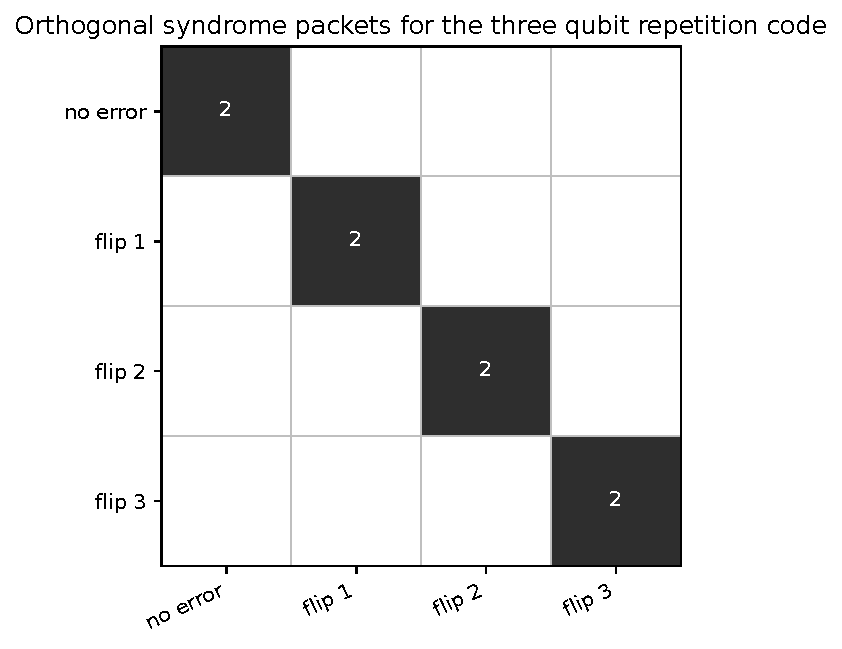
\includegraphics[width=.68\textwidth]{09_qec_syndromes.pdf}
\caption{The syndrome packets of the three qubit repetition code. Each packet has dimension two and carries the full logical state.}
\label{fig:qec_syndromes}
\end{figure}

\begin{standardfact}[Correctable observable algebras]\label{fact:operator_qec}
A finite dimensional observable algebra \(\Mcal\subseteq P\End(\Hcal)P\) is correctable for a channel with Kraus operators \((E_a)\) exactly when every compressed product \(PE_a^*E_bP\) belongs to the commutant \(\Mcal'\). The scalar code criterion is the special case \(\Mcal=P\End(\Hcal)P\) \cite{BenyKempfKribs2007}.
\end{standardfact}

\section{Feshbach effective dynamics and hidden packet memory}\label{sec:feshbach}

Let \(P\) be an orthogonal projector, put \(Q=I-P\), and write a self adjoint Hamiltonian as
\[
H=
\begin{pmatrix}
A&B\\
B^*&D
\end{pmatrix}
\]
relative to \(P\Hcal\oplus Q\Hcal\).

\begin{definition}[Feshbach map and self energy]\label{def:feshbach_map}
For \(z\notin\Spec D\), define
\[
\Sigma(z)=B(z-D)^{-1}B^*
\]
and
\[
F_P(z)=z-A-\Sigma(z).
\]
\end{definition}

\begin{theorem}[Exact projected resolvent]\label{thm:feshbach_resolvent}
If \(z\notin\Spec D\) and \(F_P(z)\) is invertible, then
\[
P(z-H)^{-1}P=F_P(z)^{-1}
\]
as an operator on \(P\Hcal\).
\end{theorem}

\begin{proof}
The lower right block of \(z-H\) is \(z-D\). Block Gaussian elimination gives
\[
\begin{pmatrix}
I&B(z-D)^{-1}\\
0&I
\end{pmatrix}
(z-H)
\begin{pmatrix}
I&0\\
(z-D)^{-1}B^*&I
\end{pmatrix}
=
\begin{pmatrix}
F_P(z)&0\\
0&z-D
\end{pmatrix}.
\]
Invert the factors and read the upper left block.
\end{proof}

\begin{theorem}[Spectral equivalence]\label{thm:feshbach_spectrum}
Let \(z\notin\Spec D\). Then
\[
z\in\Spec H
\quad\Longleftrightarrow\quad
0\in\Spec F_P(z).
\]
The map
\[
x\longmapsto
\begin{pmatrix}
x\\
(z-D)^{-1}B^*x
\end{pmatrix}
\]
is an isomorphism from \(\Ker F_P(z)\) onto \(\Ker(z-H)\).
\end{theorem}

\begin{proof}
The equation \((z-H)(x,y)^{\mathsf T}=0\) is
\[
(z-A)x-By=0,
\qquad
-B^*x+(z-D)y=0.
\]
The second equation gives \(y=(z-D)^{-1}B^*x\). Substitution into the first gives \(F_P(z)x=0\). The construction is reversible.
\end{proof}

\begin{figure}[t]
\centering
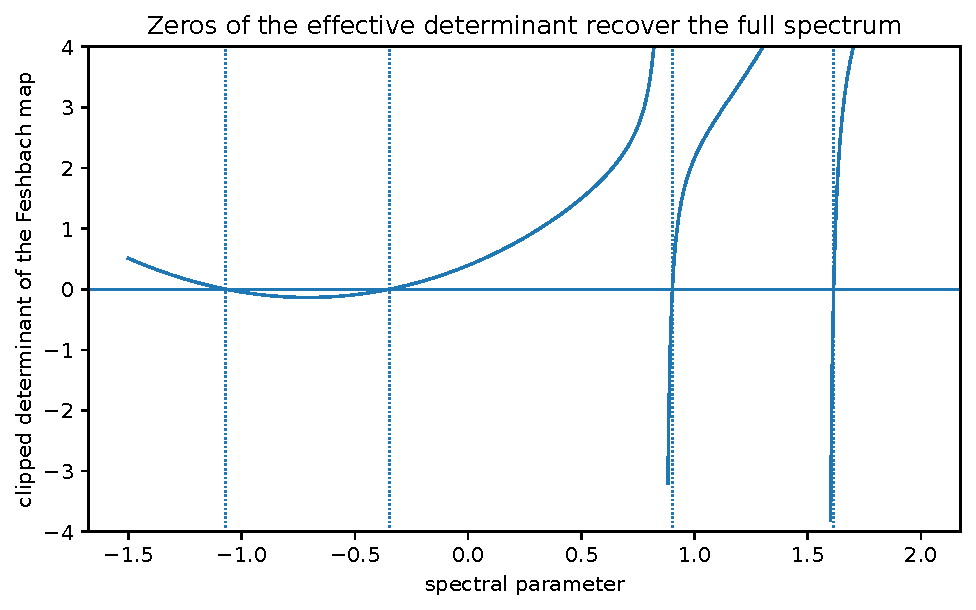
\includegraphics[width=.78\textwidth]{10_feshbach_spectrum.pdf}
\caption{The zeros of the Feshbach determinant recover the eigenvalues of the full finite Hamiltonian away from the hidden spectrum.}
\label{fig:feshbach_spectrum}
\end{figure}

\begin{theorem}[Upper half plane sign]\label{thm:self_energy_sign}
If \(\operatorname{Im}z>0\), then
\[
\operatorname{Im}\Sigma(z)
=
-(\operatorname{Im}z)
B(z-D)^{-1}(\overline z-D)^{-1}B^*
\leq0.
\]
Thus \(-\Sigma\) is an operator valued Herglotz function.
\end{theorem}

\begin{proof}
For \(R(z)=(z-D)^{-1}\), the resolvent identity gives
\[
R(z)-R(z)^*
=(\overline z-z)R(z)R(z)^*.
\]
Divide by \(2\ii\) and sandwich the result between \(B\) and \(B^*\).
\end{proof}

\begin{proposition}[Uniform self energy bounds]\label{prop:self_energy_bounds}
Let
\[
\delta=\dist(z,\Spec D)>0,
\qquad
g=\norm B.
\]
Then
\[
\norm{\Sigma(z)}\leq\frac{g^2}{\delta}
\]
and
\[
\norm{\Sigma'(z)}\leq\frac{g^2}{\delta^2}.
\]
For real \(E,E'\) in an interval at distance at least \(\delta\) from \(\Spec D\),
\[
\norm{\Sigma(E)-\Sigma(E')}
\leq
\frac{g^2}{\delta^2}\abs{E-E'}.
\]
\end{proposition}

\begin{proof}
The self adjoint resolvent satisfies
\[
\norm{(z-D)^{-1}}=\frac1{\dist(z,\Spec D)}.
\]
Differentiate the resolvent to obtain
\[
\Sigma'(z)=-B(z-D)^{-2}B^*.
\]
The first two estimates follow. The last is the mean value estimate along the real interval.
\end{proof}

\begin{proposition}[Low energy expansion]\label{prop:low_energy_expansion}
Assume \(D\) is invertible and \(\abs z\norm{D^{-1}}<1\). Then
\[
\Sigma(z)
=-
\sum_{n=0}^{\infty}
z^nBD^{-n-1}B^*
\]
with norm convergence. In particular,
\[
F_P(z)
=
 z-A+BD^{-1}B^*+O\bigl(\abs z\norm B^2\norm{D^{-1}}^2\bigr).
\]
\end{proposition}

\begin{proof}
Write
\[
(z-D)^{-1}
=-D^{-1}(I-zD^{-1})^{-1}
=-\sum_{n=0}^{\infty}z^nD^{-n-1}
\]
and sandwich by \(B\) and \(B^*\).
\end{proof}

\begin{proposition}[Bare truncation error identity]\label{prop:bare_truncation}
If both \(F_P(z)\) and \(z-A\) are invertible, then
\[
P(z-H)^{-1}P-(z-A)^{-1}
=
F_P(z)^{-1}\Sigma(z)(z-A)^{-1}.
\]
\end{proposition}

\begin{proof}
Use the inverse difference identity
\[
X^{-1}-Y^{-1}=X^{-1}(Y-X)Y^{-1}
\]
with \(X=F_P(z)\) and \(Y=z-A\).
\end{proof}

\subsection{Time memory}\label{subsec:time_memory}

Write a Schrödinger state as \(\psi=x+y\), where \(x=P\psi\) and \(y=Q\psi\).

\begin{theorem}[Exact retained memory equation]\label{thm:memory_equation}
The retained coordinate satisfies
\[
\begin{aligned}
\ii\dot x(t)
={}&Ax(t)+B\e^{-\ii tD}y(0)\\
&-\ii\int_0^tK(t-s)x(s)\dd s,
\end{aligned}
\]
where
\[
K(t)=B\e^{-\ii tD}B^*.
\]
For \(\operatorname{Re}s>0\),
\[
\int_0^\infty\e^{-st}K(t)\dd t
=
B(s+\ii D)^{-1}B^*.
\]
\end{theorem}

\begin{proof}
The hidden equation is
\[
\ii\dot y=B^*x+Dy.
\]
Variation of constants gives
\[
y(t)=\e^{-\ii tD}y(0)
-\ii\int_0^t\e^{-\ii(t-s)D}B^*x(s)\dd s.
\]
Substitute into \(\ii\dot x=Ax+By\). The Laplace formula follows by diagonalizing \(D\) or integrating the norm convergent finite dimensional exponential.
\end{proof}

\begin{theorem}[Positive definite quantum memory]\label{thm:positive_memory}
The kernel \(K(t-s)\) is positive definite. For times \(t_1,\ldots,t_m\) and retained vectors \(v_1,\ldots,v_m\),
\[
\sum_{j,k=1}^{m}
\ip{v_j}{K(t_j-t_k)v_k}
\geq0.
\]
\end{theorem}

\begin{proof}
Set
\[
w=\sum_{k=1}^{m}\e^{\ii t_kD}B^*v_k.
\]
Then
\[
\norm w^2
=
\sum_{j,k}
\ip{B^*v_j}{\e^{-\ii(t_j-t_k)D}B^*v_k}
=
\sum_{j,k}
\ip{v_j}{K(t_j-t_k)v_k}.
\]
\end{proof}

\begin{corollary}[Finite oscillatory memory expansion]\label{cor:oscillatory_memory}
If
\[
D=\sum_{r}E_rQ_r
\]
is the spectral decomposition of the hidden Hamiltonian, then
\[
K(t)=\sum_r\e^{-\ii tE_r}BQ_rB^*.
\]
Every coefficient \(BQ_rB^*\) is positive semidefinite.
\end{corollary}

\begin{proof}
Insert the spectral decomposition into the exponential.
\end{proof}

\begin{figure}[t]
\centering
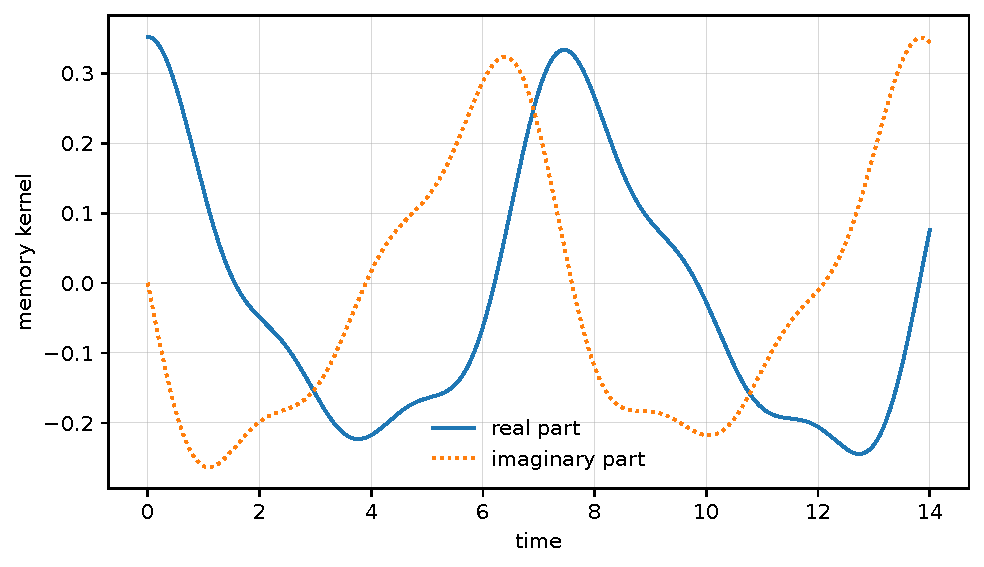
\includegraphics[width=.76\textwidth]{11_memory_kernel.pdf}
\caption{A finite hidden spectrum produces an oscillatory memory kernel rather than an instantaneous retained Hamiltonian.}
\label{fig:memory_kernel}
\end{figure}

\begin{theorem}[Exact local closure criterion]\label{thm:local_closure}
Assume \(y(0)=0\). The retained equation is local and equal to
\[
\ii\dot x=Ax
\]
for every retained initial state exactly when \(B=0\). Equivalently, exact local closure holds exactly when the retained and hidden packets reduce \(H\).
\end{theorem}

\begin{proof}
If \(B=0\), the retained and hidden equations decouple. Conversely, suppose that every solution with \(y(0)=0\) satisfies \(x(t)=\e^{-\ii tA}x(0)\). The full block equation gives
\[
\ddot x(0)
=
-\bigl(A^2+BB^*\bigr)x(0),
\]
while the declared local equation gives
\[
\ddot x(0)=-A^2x(0).
\]
Since this holds for every retained initial vector, \(BB^*=0\). Hence \(B=0\).
\end{proof}

\subsection{Stability across models}\label{subsec:feshbach_stability}

\begin{theorem}[Stability of the self energy]\label{thm:self_energy_stability}
Let
\[
\Sigma(z)=B(z-D)^{-1}B^*,
\qquad
\widetilde\Sigma(z)=\widetilde B(z-\widetilde D)^{-1}\widetilde B^*.
\]
Assume
\[
\norm B,\norm{\widetilde B}\leq g
\]
and
\[
\dist(z,\Spec D),
\dist(z,\Spec\widetilde D)
\geq\delta>0.
\]
Then
\[
\norm{\Sigma(z)-\widetilde\Sigma(z)}
\leq
\frac{2g}{\delta}\norm{B-\widetilde B}
+
\frac{g^2}{\delta^2}\norm{D-\widetilde D}.
\]
\end{theorem}

\begin{proof}
Add and subtract \(\widetilde B(z-D)^{-1}B^*\) and \(\widetilde B(z-D)^{-1}\widetilde B^*\). The first two differences give the coupling term. For the last, use
\[
(z-D)^{-1}-(z-\widetilde D)^{-1}
=(z-D)^{-1}(D-\widetilde D)(z-\widetilde D)^{-1}.
\]
Apply the resolvent bounds.
\end{proof}

\begin{corollary}[Uniform Feshbach control]\label{cor:uniform_feshbach}
For a family of packet decompositions with a common hidden spectral separation \(\delta\) and a common coupling bound \(g\), the self energies are uniformly bounded and uniformly Lipschitz on the declared spectral region. If the couplings and hidden Hamiltonians converge in norm, then the self energies converge uniformly there.
\end{corollary}

\begin{proof}
Apply \cref{prop:self_energy_bounds,thm:self_energy_stability} uniformly.
\end{proof}

This result identifies the finite hypotheses needed for cutoff independent Feshbach control. It does not prove that a chosen geometric refinement tower satisfies them.

\section{Euclidean transfer and finite reflection positivity}\label{sec:euclidean}

Let \(H=H^*\) on a finite dimensional Hilbert space and let
\[
E_0=\min\Spec H.
\]
For a lattice time step \(a>0\), define
\[
T=\e^{-a(H-E_0I)}.
\]

\begin{theorem}[Finite Euclidean transfer]\label{thm:euclidean_transfer}
The operator \(T\) is positive definite, self adjoint, and contractive. Its spectrum lies in \((0,1]\), and
\[
T^n=\e^{-na(H-E_0I)}
\]
for every \(n\in\NN\).
\end{theorem}

\begin{proof}
Diagonalize \(H\). Each eigenvalue of \(T\) is
\[
\e^{-a(E_j-E_0)}
\]
and therefore lies in \((0,1]\). The power law follows from the functional calculus.
\end{proof}

\begin{theorem}[Hamiltonian reconstruction from transfer]\label{thm:transfer_logarithm}
Let \(T\) be positive definite, self adjoint, and contractive. Then
\[
H_T=-a^{-1}\log T
\]
is a nonnegative self adjoint operator and
\[
T^n=\e^{-naH_T}.
\]
It is the unique nonnegative self adjoint operator with \(T=\e^{-aH_T}\).
\end{theorem}

\begin{proof}
Apply the real logarithm to the positive spectrum of \(T\). The spectral calculus gives existence and the power identity. Injectivity of the scalar exponential on \([0,\infty)\) gives uniqueness.
\end{proof}

\begin{theorem}[Finite reflection positivity]\label{thm:finite_reflection_positivity}
For vectors \(v_1,\ldots,v_m\in\Hcal\) and nonnegative integers \(n_1,\ldots,n_m\), the matrix
\[
G_{jk}=\ip{v_j}{T^{n_j+n_k}v_k}
\]
is positive semidefinite. Equivalently,
\[
\sum_{j,k}\overline{c_j}c_k
\ip{v_j}{T^{n_j+n_k}v_k}
\geq0
\]
for every \(c\in\CC^m\).
\end{theorem}

\begin{proof}
Since \(T\) is positive and self adjoint,
\[
\ip{v_j}{T^{n_j+n_k}v_k}
=
\ip{T^{n_j}v_j}{T^{n_k}v_k}.
\]
The quadratic form is the squared norm of
\[
\sum_kc_kT^{n_k}v_k.
\]
\end{proof}

\begin{corollary}[Reflection positive correlators]\label{cor:reflection_correlators}
Fix a vector \(\Omega\) and operators \(A_1,\ldots,A_m\). The matrix
\[
C_{jk}
=
\ip{A_j\Omega}{T^{n_j+n_k}A_k\Omega}
\]
is positive semidefinite.
\end{corollary}

\begin{proof}
Apply \cref{thm:finite_reflection_positivity} with \(v_j=A_j\Omega\).
\end{proof}

\begin{figure}[t]
\centering
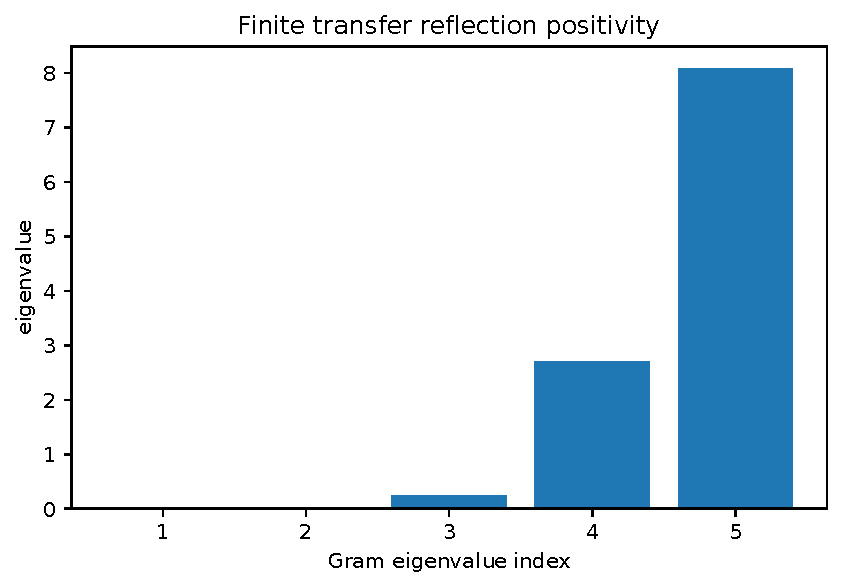
\includegraphics[width=.68\textwidth]{12_reflection_positivity.pdf}
\caption{Eigenvalues of a finite reflection positive Gram matrix. Small numerical negative values would signal either roundoff or failure of the transfer assumptions.}
\label{fig:reflection_positivity}
\end{figure}

\begin{proposition}[Ground packet convergence]\label{prop:ground_packet}
Let \(P_0\) be the spectral projector of \(H\) at \(E_0\), and let
\[
\Delta=\min\{E_j-E_0:E_j>E_0\}.
\]
If an excited eigenvalue exists, then
\[
\norm{T^n-P_0}=\e^{-na\Delta}.
\]
\end{proposition}

\begin{proof}
In the spectral decomposition, \(T^n-P_0\) has eigenvalues zero on the ground space and \(\e^{-na(E_j-E_0)}\) on the excited eigenspaces. The largest is \(\e^{-na\Delta}\).
\end{proof}

\begin{proposition}[Symmetry resolved transfer]\label{prop:symmetry_transfer}
If \([H,P_a]=0\) for a complete packet family, then
\[
T=\sum_aP_aTP_a
\]
and each reflection positive Gram matrix decomposes as the sum of its packet Gram matrices.
\end{proposition}

\begin{proof}
The functional calculus preserves commutation. Decompose every vector into packet components and use orthogonality.
\end{proof}

Finite reflection positivity is a necessary structural property of transfer data. It is not by itself the continuum Osterwalder Schrader theorem, which also requires a suitable algebra of Euclidean fields, covariance, regularity, clustering, and a controlled continuum limit \cite{OsterwalderSchrader1973,OsterwalderSchrader1975,GlimmJaffe1987}.

\section{Finite spectral geometry and diffusion dimension}\label{sec:spectral_geometry}

A finite spectral datum consists of a finite dimensional Hilbert space, a nonnegative self adjoint operator \(L\), and any declared packet family. One may take \(L=D^2\) for a finite Dirac type operator or a graph Laplacian. Related geometric viewpoints appear in \cite{Connes1994,Vassilevich2003}.

\begin{definition}[Heat trace and spectral dimension]\label{def:spectral_dimension}
Let the eigenvalues of \(L\) be \(\lambda_1,\ldots,\lambda_N\), with at least one zero eigenvalue. Define
\[
Z_L(t)=\Tr(\e^{-tL})
\]
and
\[
d_L(t)
=-2\frac{\dd\log Z_L(t)}{\dd\log t}
=
2t
\frac{\Tr(L\e^{-tL})}{\Tr(\e^{-tL})}.
\]
\end{definition}

\begin{proposition}[Finite scale limits]\label{prop:finite_spectral_limits}
For every finite nonnegative \(L\) with nontrivial kernel,
\[
\lim_{t\downarrow0}d_L(t)=0
\]
and
\[
\lim_{t\to\infty}d_L(t)=0.
\]
For every \(t>0\),
\[
0\leq d_L(t)\leq2t\norm L.
\]
\end{proposition}

\begin{proof}
The formula in \cref{def:spectral_dimension} is twice \(t\) times a weighted average of the eigenvalues. This gives the bound and the limit at zero. At large time, the denominator converges to \(\dim\Ker L\), while every positive eigenvalue contribution in the numerator decays exponentially.
\end{proof}

Thus a finite system cannot have a nonzero spectral dimension at the extreme ultraviolet or infrared ends. A geometric dimension can appear only in a refinement window.

\begin{proposition}[Heat packet decomposition]\label{prop:heat_packets}
If \([L,P_a]=0\) for every packet, then
\[
Z_L(t)=\sum_aZ_{L,a}(t),
\qquad
Z_{L,a}(t)=\Tr(P_a\e^{-tL}).
\]
The global spectral dimension is the heat weight average
\[
d_L(t)
=
\sum_a
\frac{Z_{L,a}(t)}{Z_L(t)}
 d_{L,a}(t),
\]
where
\[
d_{L,a}(t)
=2t
\frac{\Tr(P_aL\e^{-tL})}{Z_{L,a}(t)}
\]
for nonempty packet heat traces.
\end{proposition}

\begin{proof}
Commutation gives a block diagonal heat operator. Add the traces and the corresponding first spectral moments, then divide by the total heat trace.
\end{proof}

\subsection{Periodic lattices}\label{subsec:periodic_lattices}

Let \(N\geq2\) and let \(\Lambda_N=(\ZZ/N\ZZ)^d\) be the unit flat torus grid with spacing \(1/N\). The standard periodic difference Laplacian has eigenvalues
\[
\lambda_N(k)
=
4N^2
\sum_{j=1}^{d}
\sin^2\left(\frac{\pi k_j}{N}\right),
\]
where \(k\) runs through centered residue representatives. This is the standard periodic finite difference Laplacian \cite{Strikwerda2004}.

\begin{theorem}[Low mode dispersion in dimension \(d\)]\label{thm:dispersion_bound}
For every centered mode \(k\),
\[
0
\leq
4\pi^2\abs{k}^2-\lambda_N(k)
\leq
\frac{4\pi^4}{3N^2}
\sum_{j=1}^{d}k_j^4.
\]
\end{theorem}

\begin{proof}
For \(x\in[0,\pi/2]\),
\[
\sin x\leq x
\]
and
\[
\sin x\geq x-\frac{x^3}{6}.
\]
Thus
\[
0\leq x^2-\sin^2x\leq\frac{x^4}{3}.
\]
Apply this with \(x=\pi\abs{k_j}/N\), multiply by \(4N^2\), and sum over \(j\).
\end{proof}

\begin{theorem}[Fixed time heat trace convergence]\label{thm:heat_trace_convergence}
For every \(t>0\),
\[
\sum_{k\in\Lambda_N^*}
\e^{-t\lambda_N(k)}
\longrightarrow
\sum_{k\in\ZZ^d}
\e^{-4\pi^2t\abs{k}^2}
\]
as \(N\to\infty\). The first spectral moments also converge:
\[
\sum_{k\in\Lambda_N^*}
\lambda_N(k)\e^{-t\lambda_N(k)}
\longrightarrow
\sum_{k\in\ZZ^d}
4\pi^2\abs{k}^2\e^{-4\pi^2t\abs{k}^2}.
\]
Consequently, the discrete spectral dimensions converge to the continuum torus spectral dimension at every fixed positive time.
\end{theorem}

\begin{proof}
For a fixed integer mode, \cref{thm:dispersion_bound} gives
\[
\lambda_N(k)\longrightarrow4\pi^2\abs{k}^2.
\]
For centered modes, the inequality
\[
\sin x\geq\frac{2x}{\pi},
\qquad
0\leq x\leq\frac\pi2,
\]
gives
\[
\lambda_N(k)\geq16\abs{k}^2.
\]
Also \(\lambda_N(k)\leq4\pi^2\abs{k}^2\). Extend the discrete summands by zero outside the centered residue box. The heat trace terms are dominated by
\[
\e^{-16t\abs{k}^2},
\]
and the moment terms by
\[
4\pi^2\abs{k}^2\e^{-16t\abs{k}^2}.
\]
Both dominators are summable on \(\ZZ^d\). Dominated convergence proves the two limits. Their quotient gives spectral dimension convergence.
\end{proof}

\begin{standardfact}[Theta transformation]\label{fact:theta_transform}
The continuum flat torus heat trace satisfies
\[
Z_d(t)
=
\sum_{k\in\ZZ^d}\e^{-4\pi^2t\abs{k}^2}
=
(4\pi t)^{-d/2}
\sum_{n\in\ZZ^d}\e^{-\abs{n}^2/(4t)}.
\]
This is the Poisson summation formula for a Gaussian.
\end{standardfact}

\begin{theorem}[Continuum torus small time dimension]\label{thm:continuum_dimension}
Let
\[
d_{\rm torus}(t)
=-2\frac{\dd\log Z_d(t)}{\dd\log t}.
\]
Then
\[
d_{\rm torus}(t)
=
 d+O\left(t^{-1}\e^{-1/(4t)}\right)
\]
as \(t\downarrow0\).
\end{theorem}

\begin{proof}
By \cref{fact:theta_transform},
\[
Z_d(t)
=(4\pi t)^{-d/2}(1+R(t)),
\]
where
\[
R(t)=\sum_{n\neq0}\e^{-\abs{n}^2/(4t)}
=O\bigl(\e^{-1/(4t)}\bigr).
\]
Differentiation gives
\[
tR'(t)=O\left(t^{-1}\e^{-1/(4t)}\right).
\]
Insert this in the logarithmic derivative.
\end{proof}

\begin{corollary}[Rigorous intermediate dimension window]\label{cor:dimension_window}
For every \(\varepsilon>0\), there is a diffusion time \(t_\varepsilon>0\) and an integer \(N_\varepsilon\) such that
\[
\abs{d_{L_N}(t_\varepsilon)-d}<\varepsilon
\]
for every \(N\geq N_\varepsilon\).
\end{corollary}

\begin{proof}
Choose \(t_\varepsilon\) so that \cref{thm:continuum_dimension} is within \(\varepsilon/2\) of \(d\). Then apply \cref{thm:heat_trace_convergence} to choose \(N_\varepsilon\) so that the discrete spectral dimension is within \(\varepsilon/2\) of the continuum value.
\end{proof}

\begin{figure}[t]
\centering
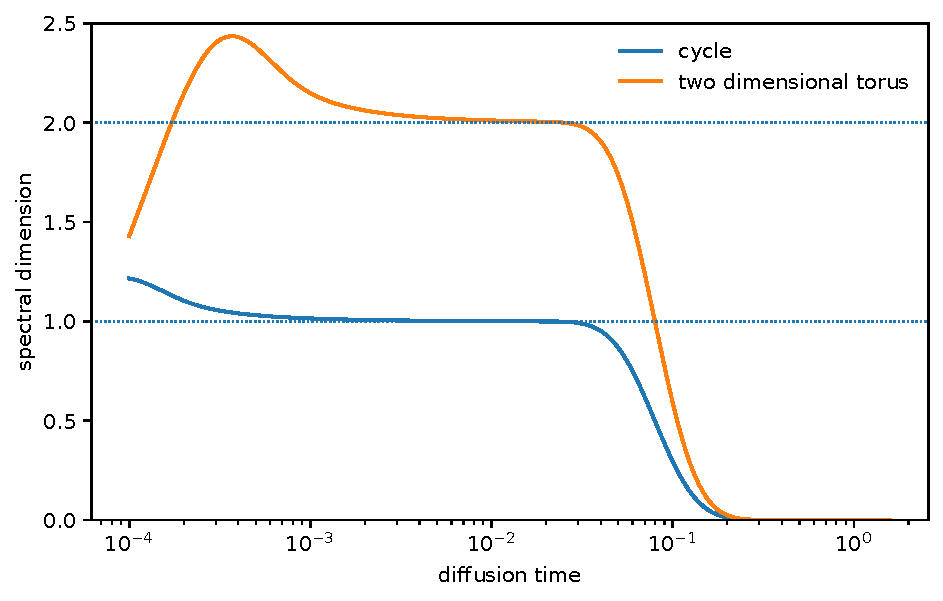
\includegraphics[width=.78\textwidth]{13_spectral_dimension.pdf}
\caption{Finite periodic lattices show an intermediate dimension window. The ultraviolet and infrared limits return to zero because the state space is finite.}
\label{fig:spectral_dimension}
\end{figure}

The order of limits matters. Taking \(t\downarrow0\) at fixed \(N\) gives zero. Taking \(N\to\infty\) at fixed positive \(t\), then taking \(t\downarrow0\), gives the continuum dimension.

\section{Constraint closure and anomaly packets}\label{sec:constraints}

Let \(C_1,\ldots,C_m\) be self adjoint constraint operators on a finite dimensional Hilbert space. The distinction between constraint action and constraint closure is standard in constrained Hamiltonian theory \cite{Dirac1964,HenneauxTeitelboim1992}. Write
\[
\mathfrak c=\operatorname{span}_{\CC}\{C_1,\ldots,C_m\}
\subseteq\End(\Hcal).
\]

\begin{definition}[Universal closure obstruction]\label{def:closure_obstruction}
Let
\[
q_{\mathfrak c}:\End(\Hcal)\longrightarrow\End(\Hcal)/\mathfrak c
\]
be the quotient map. Define
\[
\Ob_{ab}^{\rm cl}
=
q_{\mathfrak c}([C_a,C_b]).
\]
\end{definition}

\begin{theorem}[Finite constraint closure criterion]\label{thm:constraint_closure}
The constraint span \(\mathfrak c\) is closed under commutators exactly when
\[
\Ob_{ab}^{\rm cl}=0
\]
for all \(a,b\).
\end{theorem}

\begin{proof}
The quotient class vanishes exactly when \([C_a,C_b]\in\mathfrak c\). This holds for every pair exactly when \(\mathfrak c\) is a Lie algebra under the commutator.
\end{proof}

If structure coefficients \(f_{ab}^{\phantom{ab}c}\) are prescribed, define the fixed structure anomaly
\[
\mathfrak A_{ab}
=
[C_a,C_b]
-\ii\sum_cf_{ab}^{\phantom{ab}c}C_c.
\]
Exact realization of the prescribed algebra is the stronger condition \(\mathfrak A_{ab}=0\).

\begin{proposition}[Physical compression is not a closure test]\label{prop:physical_compression_trivial}
Let
\[
\Hcal_{\phys}=\bigcap_a\Ker C_a
\]
and let \(P_{\phys}\) be its orthogonal projector. Then
\[
P_{\phys}[C_a,C_b]P_{\phys}=0
\]
for every pair \(a,b\), whether or not the constraint span closes.
\end{proposition}

\begin{proof}
Self adjointness and \(C_aP_{\phys}=0\) give \(P_{\phys}C_a=0\). Both terms in the compressed commutator therefore vanish.
\end{proof}

This is why the quotient in \cref{def:closure_obstruction} is needed. Compression to physical states tests action on the common kernel, not closure of the operator algebra.

\begin{figure}[t]
\centering
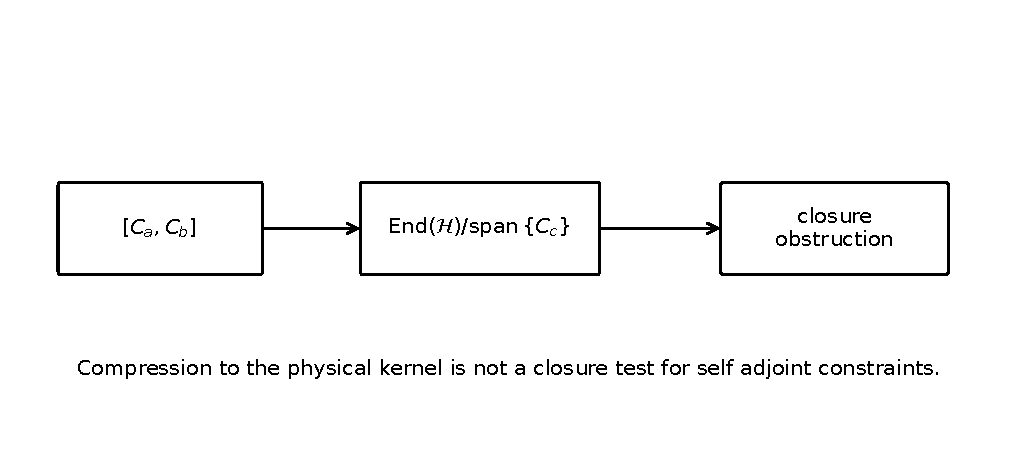
\includegraphics[width=.88\textwidth]{15_constraint_obstruction.pdf}
\caption{The closure obstruction lives in a quotient by the constraint span. Physical compression is automatic for self adjoint constraints and cannot replace this quotient.}
\label{fig:constraint_obstruction}
\end{figure}

\begin{theorem}[Invariance of the physical space]\label{thm:physical_invariance}
Let \(H=H^*\). Suppose
\[
[H,C_a]
=
\sum_cb_a^{\phantom a c}C_c
\]
for every \(a\). Then \(H\) preserves \(\Hcal_{\phys}\), and so does \(\e^{-\ii tH}\) for every real \(t\).
\end{theorem}

\begin{proof}
For \(\psi\in\Hcal_{\phys}\),
\[
C_aH\psi
=HC_a\psi-[H,C_a]\psi
=0.
\]
Thus \(H\psi\in\Hcal_{\phys}\). The exponential preserves every invariant finite dimensional subspace.
\end{proof}

\subsection{Constraint refinement}\label{subsec:constraint_refinement}

Let \((\Hcal_\ell,C_{\ell,a})\) and \((\Hcal_{\ell+1},C_{\ell+1,a})\) be two levels, and let
\[
R_\ell:\Hcal_\ell\longrightarrow\Hcal_{\ell+1}
\]
be an isometry.

\begin{theorem}[Exact constraint transport]\label{thm:constraint_transport}
Assume
\[
C_{\ell+1,a}R_\ell=R_\ell C_{\ell,a}
\]
for every \(a\). Then
\[
[C_{\ell+1,a},C_{\ell+1,b}]R_\ell
=
R_\ell[C_{\ell,a},C_{\ell,b}].
\]
If the same structure coefficients are used at both levels, then
\[
\mathfrak A_{\ell+1,ab}R_\ell
=
R_\ell\mathfrak A_{\ell,ab}.
\]
The isometry maps coarse physical states into fine physical states.
\end{theorem}

\begin{proof}
Apply the intertwining identity twice to each product in the commutator. The anomaly identity follows by subtracting the same linear combination of constraints. If \(C_{\ell,a}\psi=0\), then
\[
C_{\ell+1,a}R_\ell\psi=R_\ell C_{\ell,a}\psi=0.
\]
\end{proof}

\begin{proposition}[Approximate constraint transport]\label{prop:approx_constraint_transport}
Assume
\[
\norm{C_{\ell+1,a}R_\ell-R_\ell C_{\ell,a}}
\leq\varepsilon_a
\]
and
\[
\norm{C_{\ell,a}},\norm{C_{\ell+1,a}}\leq M.
\]
Then a coarse physical unit vector \(\psi\) satisfies
\[
\norm{C_{\ell+1,a}R_\ell\psi}\leq\varepsilon_a.
\]
Also,
\[
\begin{aligned}
&\norm{
[C_{\ell+1,a},C_{\ell+1,b}]R_\ell
-R_\ell[C_{\ell,a},C_{\ell,b}]
}\\
&\hspace{4em}\leq
2M(\varepsilon_a+\varepsilon_b).
\end{aligned}
\]
\end{proposition}

\begin{proof}
The first claim follows by applying the intertwining defect to \(\psi\). Write
\[
E_a=C_{\ell+1,a}R_\ell-R_\ell C_{\ell,a}.
\]
Expanding the two commutators gives four error terms:
\[
E_aC_{\ell,b},
\quad
C_{\ell+1,a}E_b,
\quad
-E_bC_{\ell,a},
\quad
-C_{\ell+1,b}E_a.
\]
Their norms give the bound.
\end{proof}

Approximate transport controls finite violations. It does not turn a nonzero anomaly into an exact continuum algebra without a limit theorem and a common operator domain.

\section{Quantum refinement towers}\label{sec:towers}

\begin{definition}[Finite quantum refinement tower]\label{def:quantum_tower}
A finite quantum refinement tower consists of Hilbert spaces \(\Hcal_\ell\), isometries
\[
R_\ell:\Hcal_\ell\longrightarrow\Hcal_{\ell+1},
\]
self adjoint Hamiltonians \(H_\ell\), packet projectors \(P_{\ell,a}\), constraints \(C_{\ell,r}\), and positive transfer operators \(T_\ell\). Exact compatibility means that every declared object intertwines with \(R_\ell\). Approximate compatibility is recorded by the corresponding operator norm defects.
\end{definition}

\begin{figure}[t]
\centering
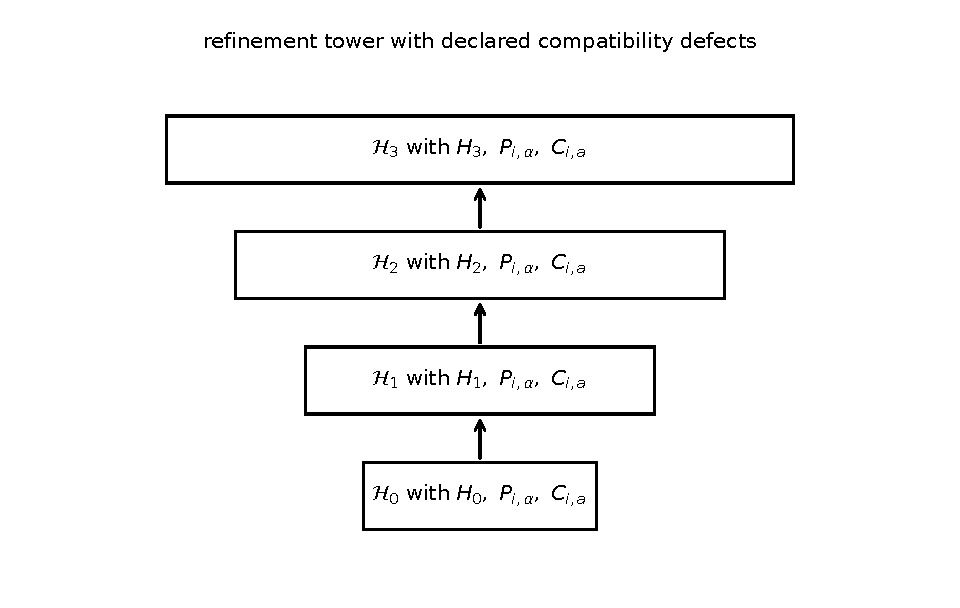
\includegraphics[width=.82\textwidth]{14_continuum_tower.pdf}
\caption{A refinement tower carries Hamiltonians, packets, constraints, and transfer data. Each family has its own compatibility defect.}
\label{fig:continuum_tower}
\end{figure}

\subsection{Exact bounded direct limits}\label{subsec:exact_direct_limit}

Let \(\Hcal_\infty\) be the Hilbert direct limit of the isometric system, and let
\[
\iota_\ell:\Hcal_\ell\longrightarrow\Hcal_\infty
\]
be the canonical isometries.

\begin{theorem}[Bounded Hamiltonian direct limit]\label{thm:bounded_direct_limit}
Assume
\[
H_{\ell+1}R_\ell=R_\ell H_\ell
\]
and
\[
\sup_\ell\norm{H_\ell}<\infty.
\]
Then there is a unique bounded self adjoint operator \(H_\infty\) on \(\Hcal_\infty\) such that
\[
H_\infty\iota_\ell=\iota_\ell H_\ell
\]
for every \(\ell\). It satisfies
\[
\e^{-\ii tH_\infty}\iota_\ell
=
\iota_\ell\e^{-\ii tH_\ell}
\]
and
\[
\e^{-tH_\infty}\iota_\ell
=
\iota_\ell\e^{-tH_\ell}
\]
when the Hamiltonians are nonnegative.
\end{theorem}

\begin{proof}
Define \(H_\infty\) on the algebraic union of the embedded levels by
\[
H_\infty\iota_\ell x=\iota_\ell H_\ell x.
\]
Compatibility makes this well defined. The uniform norm bound makes it bounded on the dense union, so it extends uniquely. It is symmetric because every \(H_\ell\) is self adjoint. A bounded symmetric operator defined on the whole Hilbert space is self adjoint. The functional calculus intertwining follows first for polynomials and then for exponentials by uniform convergence.
\end{proof}

\begin{theorem}[Exact packet direct limit]\label{thm:packet_direct_limit}
Assume each packet address \(a\) is compatible in the sense
\[
P_{\ell+1,a}R_\ell=R_\ell P_{\ell,a}.
\]
Then there is an orthogonal projector \(P_{\infty,a}\) on \(\Hcal_\infty\) satisfying
\[
P_{\infty,a}\iota_\ell=\iota_\ell P_{\ell,a}.
\]
Finite completeness and orthogonality pass to the direct limit.
\end{theorem}

\begin{proof}
Use the same construction as in \cref{thm:bounded_direct_limit}. Every projector has norm at most one, so no additional boundedness assumption is needed. The projector identities hold on the dense algebraic union and hence on the completion.
\end{proof}

\subsection{Norm summable approximation}\label{subsec:norm_summable}

The next theorem uses a common Hilbert space. It is appropriate for bounded effective Hamiltonians, not for an unbounded field Hamiltonian.

\begin{theorem}[Norm summable Hamiltonian tower]\label{thm:norm_summable_tower}
Let \((H_n)\) be bounded self adjoint operators on one Hilbert space and assume
\[
\sum_{n=0}^{\infty}\norm{H_{n+1}-H_n}<\infty.
\]
Then \(H_n\) converges in norm to a bounded self adjoint operator \(H\). For every \(T>0\),
\[
\sup_{\abs t\leq T}
\norm{\e^{-\ii tH_n}-\e^{-\ii tH}}
\leq
T\norm{H_n-H}.
\]
If every \(H_n\geq0\), then
\[
\sup_{0\leq t\leq T}
\norm{\e^{-tH_n}-\e^{-tH}}
\leq
T\norm{H_n-H}.
\]
\end{theorem}

\begin{proof}
The summability condition makes \((H_n)\) Cauchy in operator norm. The limit is self adjoint. Duhamel's identity gives
\[
\e^{-\ii tH_n}-\e^{-\ii tH}
=-\ii\int_0^t
\e^{-\ii(t-s)H_n}(H_n-H)\e^{-\ii sH}\dd s.
\]
Both unitary factors have norm one. The Euclidean estimate is identical because the nonnegative semigroups are contractions.
\end{proof}

\begin{corollary}[Limit of packet leakage]\label{cor:limit_leakage}
Let \(P_n\to P\) and \(H_n\to H\) in norm. Then for every bounded time interval,
\[
(I-P_n)\e^{-\ii tH_n}P_n
\longrightarrow
(I-P)\e^{-\ii tH}P
\]
uniformly in time.
\end{corollary}

\begin{proof}
Add and subtract terms so that one factor changes at a time. The projector terms converge uniformly because \(P_n\to P\) in norm. Duhamel's identity gives
\[
\sup_{\abs t\leq T}
\norm{\e^{-\ii tH_n}-\e^{-\ii tH}}
\leq
T\norm{H_n-H},
\]
which proves uniform convergence of the middle factor.
\end{proof}

\begin{theorem}[Reflection positivity is closed under limits]\label{thm:reflection_limit}
Suppose \(C_n(j,k)\) are reflection positive kernels on \(\NN\), meaning every finite matrix
\[
\bigl(C_n(j_r,j_s)\bigr)_{r,s}
\]
is positive semidefinite. If
\[
C_n(j,k)\longrightarrow C(j,k)
\]
for every pair, then \(C\) is reflection positive.
\end{theorem}

\begin{proof}
For a fixed finite set of times and coefficients, the corresponding quadratic forms are nonnegative and converge to the quadratic form of \(C\). The limit is nonnegative.
\end{proof}

\begin{theorem}[Constraint closure under norm convergence]\label{thm:constraint_limit}
Let \(C_{n,a}\to C_a\) in norm for every \(a\), and fix structure coefficients \(f_{ab}^{\phantom{ab}c}\). If
\[
\norm{
[C_{n,a},C_{n,b}]
-\ii\sum_cf_{ab}^{\phantom{ab}c}C_{n,c}
}
\longrightarrow0,
\]
then
\[
[C_a,C_b]
=\ii\sum_cf_{ab}^{\phantom{ab}c}C_c.
\]
\end{theorem}

\begin{proof}
Operator multiplication and the commutator are continuous in operator norm. Pass to the limit in the anomaly identity.
\end{proof}

\begin{theorem}[Heat trace convergence from trace norm]\label{thm:trace_norm_heat}
Let \(L_n,L\geq0\) act on one Hilbert space, and assume for a fixed \(t>0\) that
\[
\e^{-tL_n}\longrightarrow\e^{-tL}
\]
in trace norm. Then
\[
\Tr(\e^{-tL_n})\longrightarrow\Tr(\e^{-tL}).
\]
If also
\[
L_n\e^{-tL_n}\longrightarrow L\e^{-tL}
\]
in trace norm and the limiting heat trace is nonzero, then the spectral dimensions converge at that time.
\end{theorem}

\begin{proof}
The trace is continuous in trace norm. Apply this to the heat operators and to the first heat moments, then take the quotient in \cref{def:spectral_dimension}.
\end{proof}

\begin{remark}\label{rem:unbounded_limit}
The theorems above produce bounded continuum Hamiltonians. A physically useful continuum Hamiltonian is often unbounded. Its construction generally requires strong resolvent convergence, convergence of closed quadratic forms, or another domain sensitive method \cite{Kato1995,ReedSimon1972}. None of those conclusions follows from finite matrix convergence without additional hypotheses.
\end{remark}

\section{Continuum milestones and exact boundary}\label{sec:boundary}

The finite theorems establish exact identities and bounded limit criteria. They do not collapse the steps between a finite transfer model and a continuum theory. This section records the separate mathematical tasks.

\begin{definition}[Anomaly free continuum constraint system]\label{def:anomaly_free_continuum}
A continuum constraint system consists of a Hilbert space, a common invariant dense domain \(\Dcal\), and operators \(C_a\) on \(\Dcal\). It is anomaly free for prescribed structure coefficients when
\[
[C_a,C_b]\psi
=
\ii\sum_cf_{ab}^{\phantom{ab}c}C_c\psi
\]
for every \(\psi\in\Dcal\), and when the associated gauge evolution is defined on the physical quotient or physical subspace.
\end{definition}

Norm closure of bounded finite constraints, as in \cref{thm:constraint_limit}, is one special case. It does not treat unbounded constraints, changing domains, structure functions, or renormalized operator products.

\begin{definition}[Reflection positive Euclidean limit]\label{def:reflection_positive_limit}
A reflection positive Euclidean limit requires a limiting algebra of observables, Euclidean time translations, a reflection operation, and correlation functions whose reflected quadratic forms are nonnegative. A field theoretic reconstruction also requires the regularity and covariance assumptions needed to construct a Hilbert space, a vacuum, and a self adjoint time translation generator.
\end{definition}

\Cref{thm:reflection_limit} shows that positivity of each fixed finite Gram matrix survives pointwise convergence. It does not prove existence, locality, clustering, or the remaining Osterwalder Schrader axioms.

\begin{definition}[Einstein infrared criterion]\label{def:einstein_criterion}
A quantum geometric tower meets an Einstein infrared criterion only if a controlled long wavelength effective action exists and has an expansion whose leading geometric terms take the form
\[
\Gamma_{\rm eff}[g]
=
\int
\sqrt{\abs g}
\left(
\Lambda
+
\frac{1}{16\pi G}R
+
\text{controlled higher order terms}
\right)
\dd^dx.
\]
The expansion must respect the limiting gauge identities and must include an estimate for the omitted terms on the declared infrared regime.
\end{definition}

A spectral dimension close to four does not imply this criterion. A heat trace records eigenvalue growth. It does not determine the tensor structure, gauge identities, sign, or interaction coefficients of an effective action.

\begin{definition}[Massless spin two criterion]\label{def:spin_two_criterion}
A positive massless spin two sector requires a physical two point function or resolvent with a massless pole in the transverse traceless sector, positive residue on physical states, absence of negative norm modes, and compatibility with the limiting gauge constraints. Interactions must preserve the constraint structure.
\end{definition}

A low energy eigenvalue, a spectral dimension plateau, or a finite rank two tensor packet does not establish a massless spin two particle.

\begin{figure}[t]
\centering
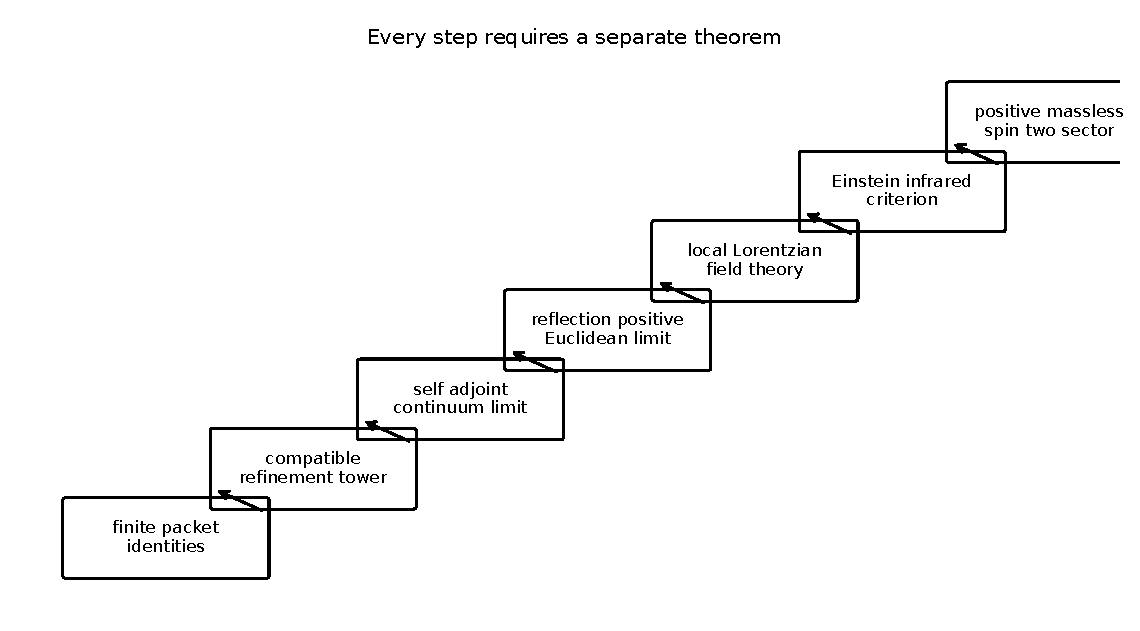
\includegraphics[width=.96\textwidth]{16_continuum_boundary.pdf}
\caption{The finite identities occupy the first step. Every later step needs a separate convergence or reconstruction theorem.}
\label{fig:continuum_boundary}
\end{figure}

\begin{table}[t]
\centering
\small
\begin{tabular}{>{\raggedright\arraybackslash}p{.25\textwidth}>{\raggedright\arraybackslash}p{.31\textwidth}>{\raggedright\arraybackslash}p{.34\textwidth}}
\toprule
Milestone & Finite result available here & Missing continuum input \\
\midrule
Symmetry and constraints & exact packets and quotient obstruction & common unbounded domain and renormalized closure \\
Effective dynamics & exact Feshbach map and uniform gap bounds & cutoff independent spectral separation and locality \\
Euclidean transfer & positive finite transfer and finite reflection positivity & convergent Euclidean fields and reconstruction axioms \\
Spectral dimension & lattice heat trace convergence & relation to a physical metric and interacting observables \\
Lorentzian theory & bounded unitary direct limits & unbounded generator, causality, locality, and field algebra \\
Einstein regime & a definition of the required expansion & derivation and error control for the effective action \\
Spin two sector & a precise spectral criterion & positive physical pole and interaction consistency \\
\bottomrule
\end{tabular}
\caption{What the finite results establish and what remains outside the article.}
\label{tab:continuum_milestones}
\end{table}

\section{Conclusion}\label{sec:conclusion}

A complete packet family gives one coordinate language for finite quantum structure. Group characters produce symmetry packets. Charged operators obey exact selection rules. Circuits become coherent sums over packet paths. The canonical moving connection separates geometric transport from physical mixing. Density matrices and channels use two sided packets, while channel covariance becomes block preservation on operator space and symmetry of the Choi matrix.

Compression to a code gives a natural error correction obstruction. Its vanishing is the Knill Laflamme condition. Diagonalizing the resulting coefficient matrix produces orthogonal syndrome packets and an exact recovery on the error span. Schur Feshbach elimination gives an equally exact description of hidden Hamiltonian packets. Their frequency response is the self energy, and their time response is a positive definite memory kernel.

Positive Euclidean transfer gives finite reflection positivity. Periodic lattice heat traces converge to the continuum torus at every fixed positive diffusion time, and the continuum small time spectral dimension is recovered after the refinement limit. Constraint closure is measured by a quotient of operator space, not by compression to the physical kernel.

The bounded tower theorems show how exact compatibility and norm summability produce limiting quantum evolutions. They also show the boundary of the argument. Unbounded field Hamiltonians, continuum gauge constraints, reflection positive field measures, the Einstein infrared action, and a massless spin two sector require additional theorems. The finite packet calculus organizes those questions but does not settle them.

\section*{Language model contribution}

An OpenAI language model was used to help reorganize the original finite manuscript, test alternative formulations, draft parts of the exposition, and design finite verification calculations. Its mathematical suggestions affected the finite group projector section, the moving packet leakage estimate, the operator space channel decomposition, the compression obstruction for error correction, the self energy estimates, the spectral dimension limit, and the quotient formulation of constraint closure. The author is responsible for checking every statement, proof, citation, and computation in any submitted version. The model is not an author.

\bibliographystyle{amsplain}
\bibliography{PSC_Paper_VII_Strengthened_Annals_Edition}

\end{document}
